% Build from reports/: latexmk -xelatex -interaction=nonstopmode -halt-on-error main.tex
\documentclass[UTF8,a4paper,zihao=-4,fontset=fandol]{ctexart}
\usepackage[margin=2.5cm]{geometry}
\usepackage{amsmath,amssymb,booktabs,graphicx,setspace,tabularx}
\usepackage{tikz}
\usetikzlibrary{arrows.meta,positioning}
\usepackage[font=small,labelfont=bf]{caption}
\usepackage[section]{placeins}
\usepackage[numbers,sort&compress]{natbib}
\usepackage{fvextra}
\usepackage[unicode,hidelinks]{hyperref}
\setstretch{1.25}
\setlength{\textfloatsep}{12pt plus 2pt minus 2pt}
\setlength{\floatsep}{10pt plus 2pt minus 2pt}
\setlength{\abovecaptionskip}{5pt}
\setlength{\belowcaptionskip}{4pt}
\setcounter{topnumber}{3}
\renewcommand{\topfraction}{0.9}
\renewcommand{\textfraction}{0.08}
\emergencystretch=2em
\numberwithin{equation}{section}
\numberwithin{figure}{section}
\numberwithin{table}{section}
\graphicspath{{figures/}{../figures/}}
\title{GraphMAE的部分复现与度数感知掩码实验分析}
\author{机器学习课程大作业（姓名及学号待填写）}
\date{\today}
% M3.3：完整附录已接入；从reports目录编译完整解压后的工程。
\newif\ifincludeFullAppendix
\includeFullAppendixtrue
\newcommand{\appendixfile}[1]{%
  \VerbatimInput[fontsize=\fontsize{7.5}{9}\selectfont,numbers=left,
  numbersep=5pt,breaklines=true,breakanywhere=true,tabsize=2]{\detokenize{#1}}}
\newcommand{\appendixtext}[1]{%
  \VerbatimInput[fontsize=\fontsize{8.5}{10}\selectfont,
  breaklines=true,breakanywhere=true,tabsize=2]{\detokenize{#1}}}
\begin{document}
\maketitle
\begin{abstract}
GraphMAE通过掩码节点特征重建学习图表示，以GNN解码器、重掩码和缩放余弦误差缓解平凡重建问题。
本文基于锁定的官方PyG实现，在Cora公开划分上完成五随机种子的部分复现，测试准确率为83.98\%，样本标准差为1.056882个百分点。
进一步设计度数感知掩码，在保持每轮1354个掩码节点及其余配置不变的条件下，以$(d_i+1)^{\alpha_d}$进行加权无放回采样。
对$\alpha_d\in\{0,0.25,0.5,1\}$各运行五个种子，仅依据验证集选择最佳正向系数0.25后进行最终测试。
控制组与所选方案的测试均值分别为84.20\%和82.92\%，平均配对变化为$-1.28$个百分点。
度数加权提高了高度数节点的实际掩码频率，但三类度数组的平均分类准确率均下降，未支持本次性能改善假设。
实验仅涉及单一数据集及五个种子，结果用于分析采样偏置与下游任务的关系，不构成策略普遍无效的证明。
\end{abstract}
\noindent\textbf{关键词：}图自监督学习；GraphMAE；特征重建；度数感知掩码；节点分类
\section{引言}\label{sec:introduction}
图表示学习将节点属性与关系结构映射为可用于分类等任务的向量。与独立同分布样本不同，图中节点的预测依赖其自身特征和邻域信息；但获取节点类别标签通常需要额外成本，少量标签难以直接覆盖图的复杂结构。图神经网络可通过邻域聚合联合利用结构与属性，图自监督学习则进一步从未标注数据中构造训练信号，再将所得表示用于下游任务。

GraphMAE是Hou等发表于KDD 2022的生成式图自监督方法\cite{hou2022graphmae}。它关注一个具体问题：如何使图自编码器学到有用表示，而不是仅完成容易的输入复制或结构拟合？其设计以节点特征为重建目标，通过输入掩码、图神经网络解码、解码前重掩码及缩放余弦误差形成自监督任务。结构仍用于消息传递，但不被作为该重建损失的预测对象。本文选择该论文开展课程级部分复现，范围限定为Cora上的节点分类，不覆盖原论文的全部数据集和任务。

本文的工作包括两部分。首先，固定官方代码版本、数据处理和超参数，完成五种子复现，并将验证集选模与测试集最终评价分离。其次，提出并检验度数感知掩码假设：高度数节点具有较多邻域上下文，提高其掩码频率是否有助于表示学习？为此只调整掩码节点选择分布，在固定预算下对三个正向系数和均匀控制组进行配对实验。GraphMAE本身的架构与损失贡献属于原作者；本文的自主工作是采样适配、随机数流控制及相应实验分析。实验并未获得平均分类性能提升，因此本文保留负结果，并分析其证据边界。

\section{相关研究}\label{sec:related}
\subsection{图神经网络与图注意力}
GCN将节点特征变换与归一化邻域聚合结合，用于半监督节点分类\cite{kipf2017gcn}。GAT通过邻域内的注意力归一化分配不同邻居的聚合权重，并用多头机制组合表示\cite{velickovic2018gat}。二者说明拓扑与属性可共同进入节点编码。本文采用GraphMAE官方实现中的GAT，不重新选择骨干；GAT内部的注意力权重服务于消息传递，与本文按度数选择训练目标的掩码权重处于不同层次。

\subsection{图自监督的对比式与生成式路线}
图自监督可以通过区分相匹配与受扰动的表示构造目标，也可以通过恢复输入信息进行训练。DGI将局部节点表示与全图摘要联系起来，并通过受扰动图构造对照信号，以互信息最大化思想学习表示\cite{velickovic2019dgi}。这类方法的关键在于构造有效的正负关系；不同方法对增强和训练过程的要求不尽相同，不能将其概括为同一种实现。

生成式方法则明确指定重建对象。例如VGAE使用GCN编码器和内积解码器完成图链接预测\cite{kipf2016vgae}。GraphMAE转向节点特征恢复，并不认为所有图任务都必须首先重建邻接矩阵。重建目标是否适合下游任务、解码器是否能迫使编码器提取有用信息，是两类方法比较时需要区分的因素。

\subsection{掩码自编码与GraphMAE}
BERT通过预测受遮蔽的文本内容开展预训练\cite{devlin2019bert}；视觉MAE使用仅处理可见图像块的编码器和恢复像素的解码器\cite{he2022mae}。二者为从部分观测恢复输入提供了不同领域的例子。GraphMAE沿用掩码重建思想，但适应图数据的邻域依赖：被掩码节点仍进入整图编码，采用GNN解码器，并在解码前重新遮蔽同一批节点的隐表示。其SCE直接衡量特征方向误差，避免将图节点特征机械地视为文本离散词元或图像像素。

本文的度数策略不改变上述信息流，而是改变哪些节点更频繁地成为重建目标。原论文已经指出均匀采样有助于减少邻域观测偏置。因此，偏向高度数节点既有更多上下文可用的动机，也存在破坏上下文与减少低度数监督的风险，需要在统一训练配置下检验。

\section{GraphMAE算法原理}\label{sec:method}
\subsection{问题定义与整体信息流}
设无向属性图为$G=(V,E,X)$，$N=|V|$为节点数，$A\in\{0,1\}^{N\times N}$为邻接矩阵，$X\in\mathbb R^{N\times F}$为节点特征矩阵，$x_i\in\mathbb R^F$表示第$i$个节点的特征向量。预训练不使用类别标签，目标是学习编码器$f_E$，使其表示可支持少量标注下的节点分类。图\ref{fig:graphmae}展示官方流程。后文公式采用列向量描述单个节点，用矩阵的行堆叠表示整图。

\begin{figure}[tbp]
\centering
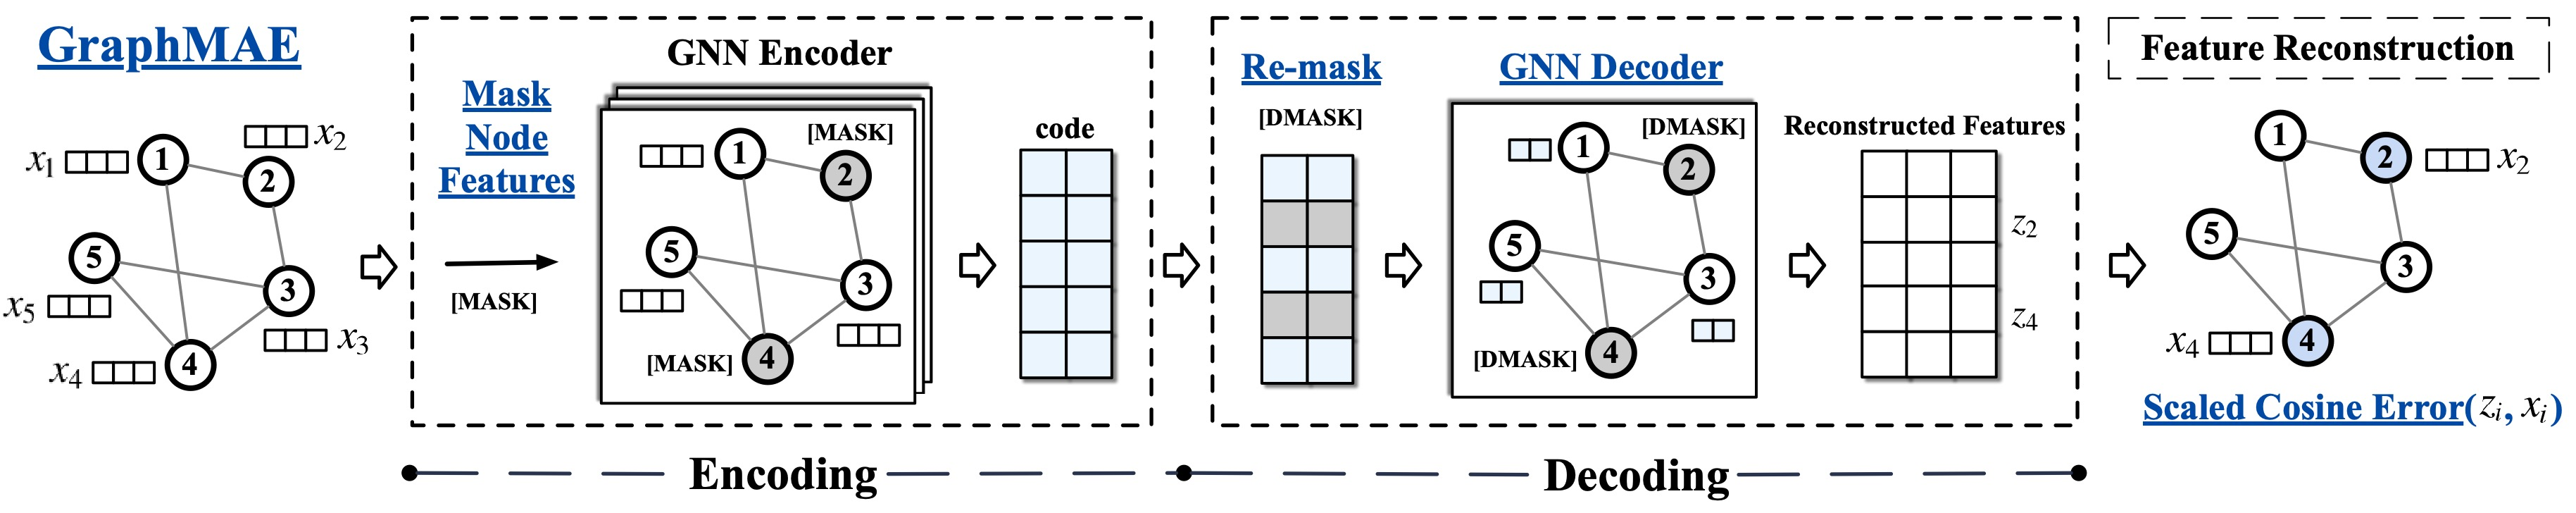
\includegraphics[width=\linewidth]{figures/graphmae_official.jpg}
\caption{GraphMAE整体流程。图片直接取自官方仓库，内容对应原论文图2中的GraphMAE部分\cite{hou2022graphmae}，并非本文新设计的架构。输入特征经掩码、GNN编码、重掩码与GNN解码后，在被选节点上计算SCE。锁定Cora实现中重掩码使用零向量。}
\label{fig:graphmae}
\end{figure}

模型的输入是图结构及部分可见特征，输出是重建特征$Z\in\mathbb R^{N\times F}$。本文计算图采用先去自环、再逐节点加一次自环的邻接关系$\bar A$。结构用于编码和解码的邻域聚合，并未作为预测目标引入边重建损失。

\subsection{节点特征掩码与随机替换}
设掩码比例为$r$，原始策略每轮均匀、无放回选择集合$M$：
\begin{equation}\label{eq:uniform}
k=\lfloor rN\rfloor,\quad M\subset V,\quad |M|=k,\qquad
M\sim\operatorname{UniformWithoutReplacement}(V,k).
\end{equation}
各节点的边际纳入概率为$k/N$。这里遮蔽的是节点特征，节点及关联边仍保留，故编码器可沿图结构传播信息。对Cora，$N=2708,r=0.5$，每轮选择1354个不同节点。

原论文的基本描述是用可学习向量$x_{\rm mask}$替换选中节点特征。实际配置还对少量选中节点随机替换为其他节点特征，以缓和预训练与无掩码推断的差异。设$T\subset M$为mask token节点、$R\subset M$为随机替换节点，$T\cap R=\varnothing$，则
\begin{equation}\label{eq:corruption}
\widetilde x_i=\begin{cases}
x_{\rm mask},& i\in T,\\
x_{j(i)},& i\in R,\\
x_i,& \text{其他},
\end{cases}
\end{equation}
其中$j(i)$为随机选取的特征供体节点，$x_{\rm mask}\in\mathbb R^F$初始为零并参加梯度更新。锁定源码分别计算$|T|=\lfloor(1-q)k\rfloor$和$|R|=\lfloor qk\rfloor$，$q=0.05$。因此1354个选中节点中1286个使用token，67个随机替换，另1个因两次取整而保留原特征；它仍属于$M$，参加后续重掩码与损失计算。本文保留这一实现细节，没有将其改成新的扰动比例。

\subsection{GAT编码器}
编码器计算$H=f_E(\bar A,\widetilde X)$。令$h_i^{(l)}$为第$l$层节点表示，初值$h_i^{(0)}=\widetilde x_i$；第$a$个注意力头采用投影矩阵$W^{(l,a)}$和源、目标注意力向量$u_{\rm src}^{(l,a)},u_{\rm dst}^{(l,a)}$。省略Dropout时，边$j\to i$的打分和邻域归一化为
\begin{align}
e_{ij}^{(l,a)}&=\operatorname{LeakyReLU}\!\left[
(u_{\rm dst}^{(l,a)})^{\mathsf T}W^{(l,a)}h_i^{(l)}+
(u_{\rm src}^{(l,a)})^{\mathsf T}W^{(l,a)}h_j^{(l)}\right],\label{eq:attention-score}\\
\beta_{ij}^{(l,a)}&=\frac{\exp(e_{ij}^{(l,a)})}
{\sum_{v\in\mathcal N(i)\cup\{i\}}\exp(e_{iv}^{(l,a)})}.\label{eq:attention-weight}
\end{align}
邻域$\mathcal N(i)$不含节点自身，额外的$\{i\}$对应自环。用$K$个头拼接并加入偏置，可写出层更新：
\begin{equation}\label{eq:gat-update}
h_i^{(l+1)}=\sigma\!\left[
\mathop{\Vert}_{a=1}^{K}\left(\sum_{j\in\mathcal N(i)\cup\{i\}}
\beta_{ij}^{(l,a)}W^{(l,a)}h_j^{(l)}\right)+b^{(l)}\right].
\end{equation}
符号$\Vert$表示拼接，$b^{(l)}$为拼接后的偏置，$\sigma$为激活函数。训练时每层投影前对输入特征做Dropout，softmax后对注意力系数做Dropout；此时实际用于聚合的系数不必再严格和为1。Cora编码器使用两层GAT，每层4头、每头128维，总输出512维，激活为PReLU；特征与注意力Dropout分别为0.2、0.1，LeakyReLU斜率0.2，不使用残差和归一化层。式\eqref{eq:attention-score}--\eqref{eq:gat-update}对应官方自定义PyG消息传递实现，而非任意默认配置的GAT模块。

\subsection{线性映射、Re-mask与解码器}
编码后先用无偏置线性层将表示映射到解码输入空间，再将同一个$M$内节点的表示置零：
\begin{equation}\label{eq:remask}
H=f_E(\bar A,\widetilde X),\quad Q=HW_{ED},\qquad
\widetilde q_i=\begin{cases}0,&i\in M,\\q_i,&i\notin M,\end{cases}
\quad Z=f_D(\bar A,\widetilde Q).
\end{equation}
其中$W_{ED}\in\mathbb R^{512\times512}$，$H,Q,\widetilde Q\in\mathbb R^{N\times512}$。原论文以解码掩码token描述Re-mask，式\eqref{eq:remask}按本次锁定源码具体写为零向量。它阻止解码器直接读取被掩码节点自身的编码表示，促使其借助邻居恢复特征；但邻居编码已融合过局部信息，因此不能理解为消除了所有关于这些节点的间接信号。

解码器是一层GAT，以1个输出头恢复$F=1433$维特征，最后一层不使用编码器的PReLU激活。其结构在本次Cora实现中固定，不随编码器两层设置而变成两层。表\ref{tab:dimensions}给出张量维度。下游推断只保留编码器，不使用投影层、Re-mask或解码器。
\begin{table}[tbp]
\centering\small
\caption{Cora路径中的主要张量与模块维度。}\label{tab:dimensions}
\begin{tabular}{lll}\toprule
对象/模块 & 输入 & 输出\\\midrule
掩码前后特征$X,\widetilde X$ & $2708\times1433$ & $2708\times1433$\\
GAT编码第1层 & $2708\times1433$ & $2708\times(4\times128)$\\
GAT编码第2层 & $2708\times512$ & $2708\times(4\times128)$\\
无偏置投影与Re-mask & $2708\times512$ & $2708\times512$\\
单层GAT解码器 & $2708\times512$ & $2708\times(1\times1433)$\\
下游线性分类器 & $2708\times512$ & $2708\times7$\\\bottomrule
\end{tabular}
\end{table}

\subsection{缩放余弦误差}
原论文提出缩放余弦误差（Scaled Cosine Error，SCE）作为特征恢复目标。令$z_i$为重建向量，$\gamma\ge1$为缩放指数，损失只在$M$上计算：
\begin{equation}\label{eq:sce}
\mathcal L_{\rm SCE}=\frac1{|M|}\sum_{i\in M}
\left(1-\frac{x_i^{\mathsf T}z_i}{\|x_i\|_2\|z_i\|_2}\right)^\gamma.
\end{equation}
该式对应原论文式(2)。实现先沿特征维做$\ell_2$归一化，范数分母使用epsilon保护，再计算余弦误差的幂及均值。与直接MSE相比，归一化减弱向量尺度对目标的影响；当余弦误差小于1时，较大的指数会更快降低易例的贡献，但不能据此声称所有误差均被缩小。Cora设$\gamma=3$，代码参数名为\texttt{alpha\_l}，与后文采样指数$\alpha_d$无关。

\subsection{预训练与冻结线性评估}
预训练以全图特征扰动后的SCE优化编码器、投影、解码器和mask token，不接收类别标签。完成后用无掩码特征生成冻结表示$U=f_E(\bar A,X)\in\mathbb R^{N\times512}$。线性分类器以$W_c\in\mathbb R^{512\times C}$及偏置$b_c\in\mathbb R^C$产生类别概率：
\begin{equation}\label{eq:classifier}
P=\operatorname{softmax}(UW_c+\mathbf1 b_c^{\mathsf T}),\qquad
\mathcal L_{\rm cls}=-\frac1{|V_{\rm tr}|}\sum_{i\in V_{\rm tr}}\log P_{i,y_i}.
\end{equation}
$C=7$，$y_i$为训练标签，$V_{\rm tr}$为训练节点集；实现中交叉熵直接接受logits，不显式先做softmax。encoder在这一阶段不更新。最终Probe完整训练300轮后，按验证准确率选择分类器：
\begin{equation}\label{eq:probe-selection}
t^*=\max\arg\max_{1\le t\le300}\operatorname{Acc}_{\rm val}(t).
\end{equation}
外层$\max$表示验证平分时保留较晚轮，与官方\texttt{>=}规则一致。测试标签仅在选模完成后用于最终评分；具体预训练和周期Probe协议见第\ref{sec:protocol}节。

\section{实验环境与复现方案}\label{sec:protocol}
\subsection{实现来源与运行环境}
正式实现来自官方仓库\url{https://github.com/THUDM/GraphMAE}的PyG分支，固定Commit为\texttt{9127f25e01aa5ba1cca68b746284aeb7ab2b4850}。本文没有修改第三方源码，而是在独立包装器中处理配置、日志、掩码适配与标签隔离。官方DGL主分支仅作静态审计，没有作为第二套数值复现。表\ref{tab:environment}列出主要环境，完整依赖锁随项目保留。
\begin{table}[tbp]
\centering\small
\caption{实验环境与原论文环境的区别。}\label{tab:environment}
\begin{tabularx}{\linewidth}{lXX}\toprule
项目 & 本项目 & 原论文节点分类环境\\\midrule
系统/CPU & Ubuntu 24.04.4；双路Xeon Gold 5320 & Linux；Xeon E5-2680 v4等\\
GPU & M1：A40；M2训练：L40 & Cora等主要实验：RTX 2080Ti\\
Python / PyTorch & 3.11.7 / 2.4.1+cu121 & 3.7 / 1.9.0\\
图学习框架 & PyG 2.3.1 & DGL 0.7.2\\
CUDA & PyTorch运行库12.1 & 10.2\\
数值/评估库 & NumPy 1.26.4；sklearn 1.5.2 & sklearn 0.24.1\\\bottomrule
\end{tabularx}
\end{table}
系统驱动为595.91.07，系统CUDA Toolkit为13.2.51；它们与PyTorch实际使用的12.1运行库不是同一概念。M1五次训练均使用物理GPU2 A40，M2二十次训练使用物理GPU0 L40；按UUID设置可见设备后，进程内部均为\texttt{cuda:0}。M2最后一个模型的测试推断迁至A40，具体限制见第\ref{sec:limitations}节。实验在项目独立Python环境中运行，未混用其他项目的模型依赖。

\subsection{Cora数据与传导学习协议}
Cora包含2708个节点、1433维节点特征和7个类别。采用官方PyG的Planetoid加载路径和public split，训练、验证、测试节点数分别为140、500、1000，三者互不交叠；其余1068个节点不参与有监督标签训练。非负特征使用NormalizeFeatures逐行归一化，删除原有自环后给每个节点添加一个自环。

本项目处理后的图有10556个非自环有向边条目，双向对称且无非自环重复，对应5278个唯一无向邻居对；添加2708个自环后共13264个边条目。原论文数据表列出5429条边，不能将其与上述处理后条目直接混用。本文以实际缓存、预处理和SHA256校验记录定义复现数据，不推断这一计数差异的未核实原因。M0、M1、M2共用的8个raw及3个processed文件校验一致。

实验采用传导学习（transductive）设置：预训练可以访问整张图的结构与特征，包括测试节点特征，但不使用类别标签。线性Probe只用140个训练标签更新参数，以500个验证标签选择分类器；测试标签不参与训练、配置调整或选择。M0的20轮短测仅证明流程可运行，不加入正式统计。

\subsection{固定配置与评估流程}
表\ref{tab:hyperparameters}采用官方\texttt{configs.yml}的Cora有效配置。加载后保存实际参数，核对同值重复键的解析结果；解码层数由模型构造固定为1。M1与M2除掩码选择随机协议外共用该表配置，没有为接近论文结果额外调参。
\begin{table}[tbp]
\centering\small
\caption{M1与M2共用的训练配置。}\label{tab:hyperparameters}
\begin{tabularx}{\linewidth}{lXlX}\toprule
参数 & 设置 & 参数 & 设置\\\midrule
Encoder & 2层GAT，4头，512维 & Decoder & 1层GAT，1输出头\\
Mask / Replace & 0.5 / 0.05 & SCE指数$\gamma$ & 3（\texttt{alpha\_l}）\\
特征/注意力Dropout & 0.2 / 0.1 & Drop edge & 0\\
优化器 & Adam & 学习率调度 & Cosine\\
预训练学习率 & 0.001 & 预训练权重衰减 & 0.0002\\
预训练轮数 & 1500 & 每次Probe轮数 & 300\\
Probe学习率 & 0.01 & Probe权重衰减 & 0.0001\\
Encoder激活 & PReLU & 残差/归一化 & 均不使用\\\bottomrule
\end{tabularx}
\end{table}

每次预训练保留官方在第200、400、600、800、1000、1200和1400轮进行的七次线性Probe，每次完整300轮。这些Probe只评价验证集，不用于选择encoder；其初始化与更新消耗的随机数不被隔离。encoder固定取第1500轮，随后重新训练最终300轮分类器，按式\eqref{eq:probe-selection}选定权重后测试一次。包装器移除了官方周期评估中的测试指标计算，但保留分类器、Adam、训练更新与验证平分规则。测试集没有参与选模。

\subsection{随机性与统计方法}
五个随机种子固定为0、1、2、3、4，各次独立进程顺序执行。入口设置Python、NumPy、PyTorch CPU/CUDA种子，令cuDNN deterministic为真、benchmark为假；未强制启用可能不兼容的完全确定性算法。GPU scatter等归约仍可能产生非位级确定性。

设测试节点集为$V_{\rm te}$，预测类别为$\widehat y_i$，则
\begin{equation}\label{eq:accuracy}
a_s=\operatorname{Acc}_s=\frac1{|V_{\rm te}|}\sum_{i\in V_{\rm te}}\mathbf1\{\widehat y_i=y_i\},\quad
\bar a=\frac15\sum_{s=0}^{4}a_s,\quad
s_a=\sqrt{\frac1{4}\sum_{s=0}^{4}(a_s-\bar a)^2}.
\end{equation}
其中$\mathbf1$为指示函数，下标$s$表示种子。本文报告均值及样本标准差（ddof=1），把比例乘100后，均值以百分比表示，标准差和差值以百分点表示。Cora为单标签多分类，所有类别计入时Micro-F1与Accuracy相同，故不把两者作为独立效果证据。图中误差条和波动带均为跨五种子的样本标准差，不是置信区间。

\section{GraphMAE原始算法复现}\label{sec:reproduction}
\subsection{五种子结果与训练过程}
表\ref{tab:m1}保留五次正式运行的全部结果。每次均完成1500轮预训练、七次周期Probe和300轮最终Probe，没有提前停止。选中轮次只指最终分类器的验证最优轮次，例如seed4选择第25轮，并不表示只训练了25轮。
\begin{table}[tbp]
\centering\small
\caption{M1原始GraphMAE复现。Accuracy单位为\%，时间为独立worker总耗时，包含导入、数据加载、全部训练/Probe及保存。}\label{tab:m1}
\begin{tabular}{rrrrr}\toprule
Seed & 最佳验证Accuracy & 分类器选中轮次 & 测试Accuracy & 时间/s\\\midrule
0 & 79.80 & 300 & 84.40 & 27.082\\
1 & 79.60 & 300 & 84.50 & 26.497\\
2 & 80.40 & 193 & 83.90 & 25.738\\
3 & 80.60 & 153 & 84.90 & 25.312\\
4 & 80.00 & 25 & 82.20 & 25.832\\\midrule
均值 & 80.08 & --- & 83.98 & 26.092\\\bottomrule
\end{tabular}
\end{table}

图\ref{fig:m1-loss}显示SCE由接近1的初始水平下降，并逐渐进入约0.4量级的波动区间。训练中每轮重新抽取掩码且使用Dropout，故局部起伏并不意味着训练中断。五次训练Loss均为有限值，日志、有效配置、每轮学习率、最佳分类器及最终预训练权重均保留。损失曲线表明重建任务得到优化，但分类表现仍须通过冻结表示的Probe判断。
\begin{figure}[tbp]
\centering
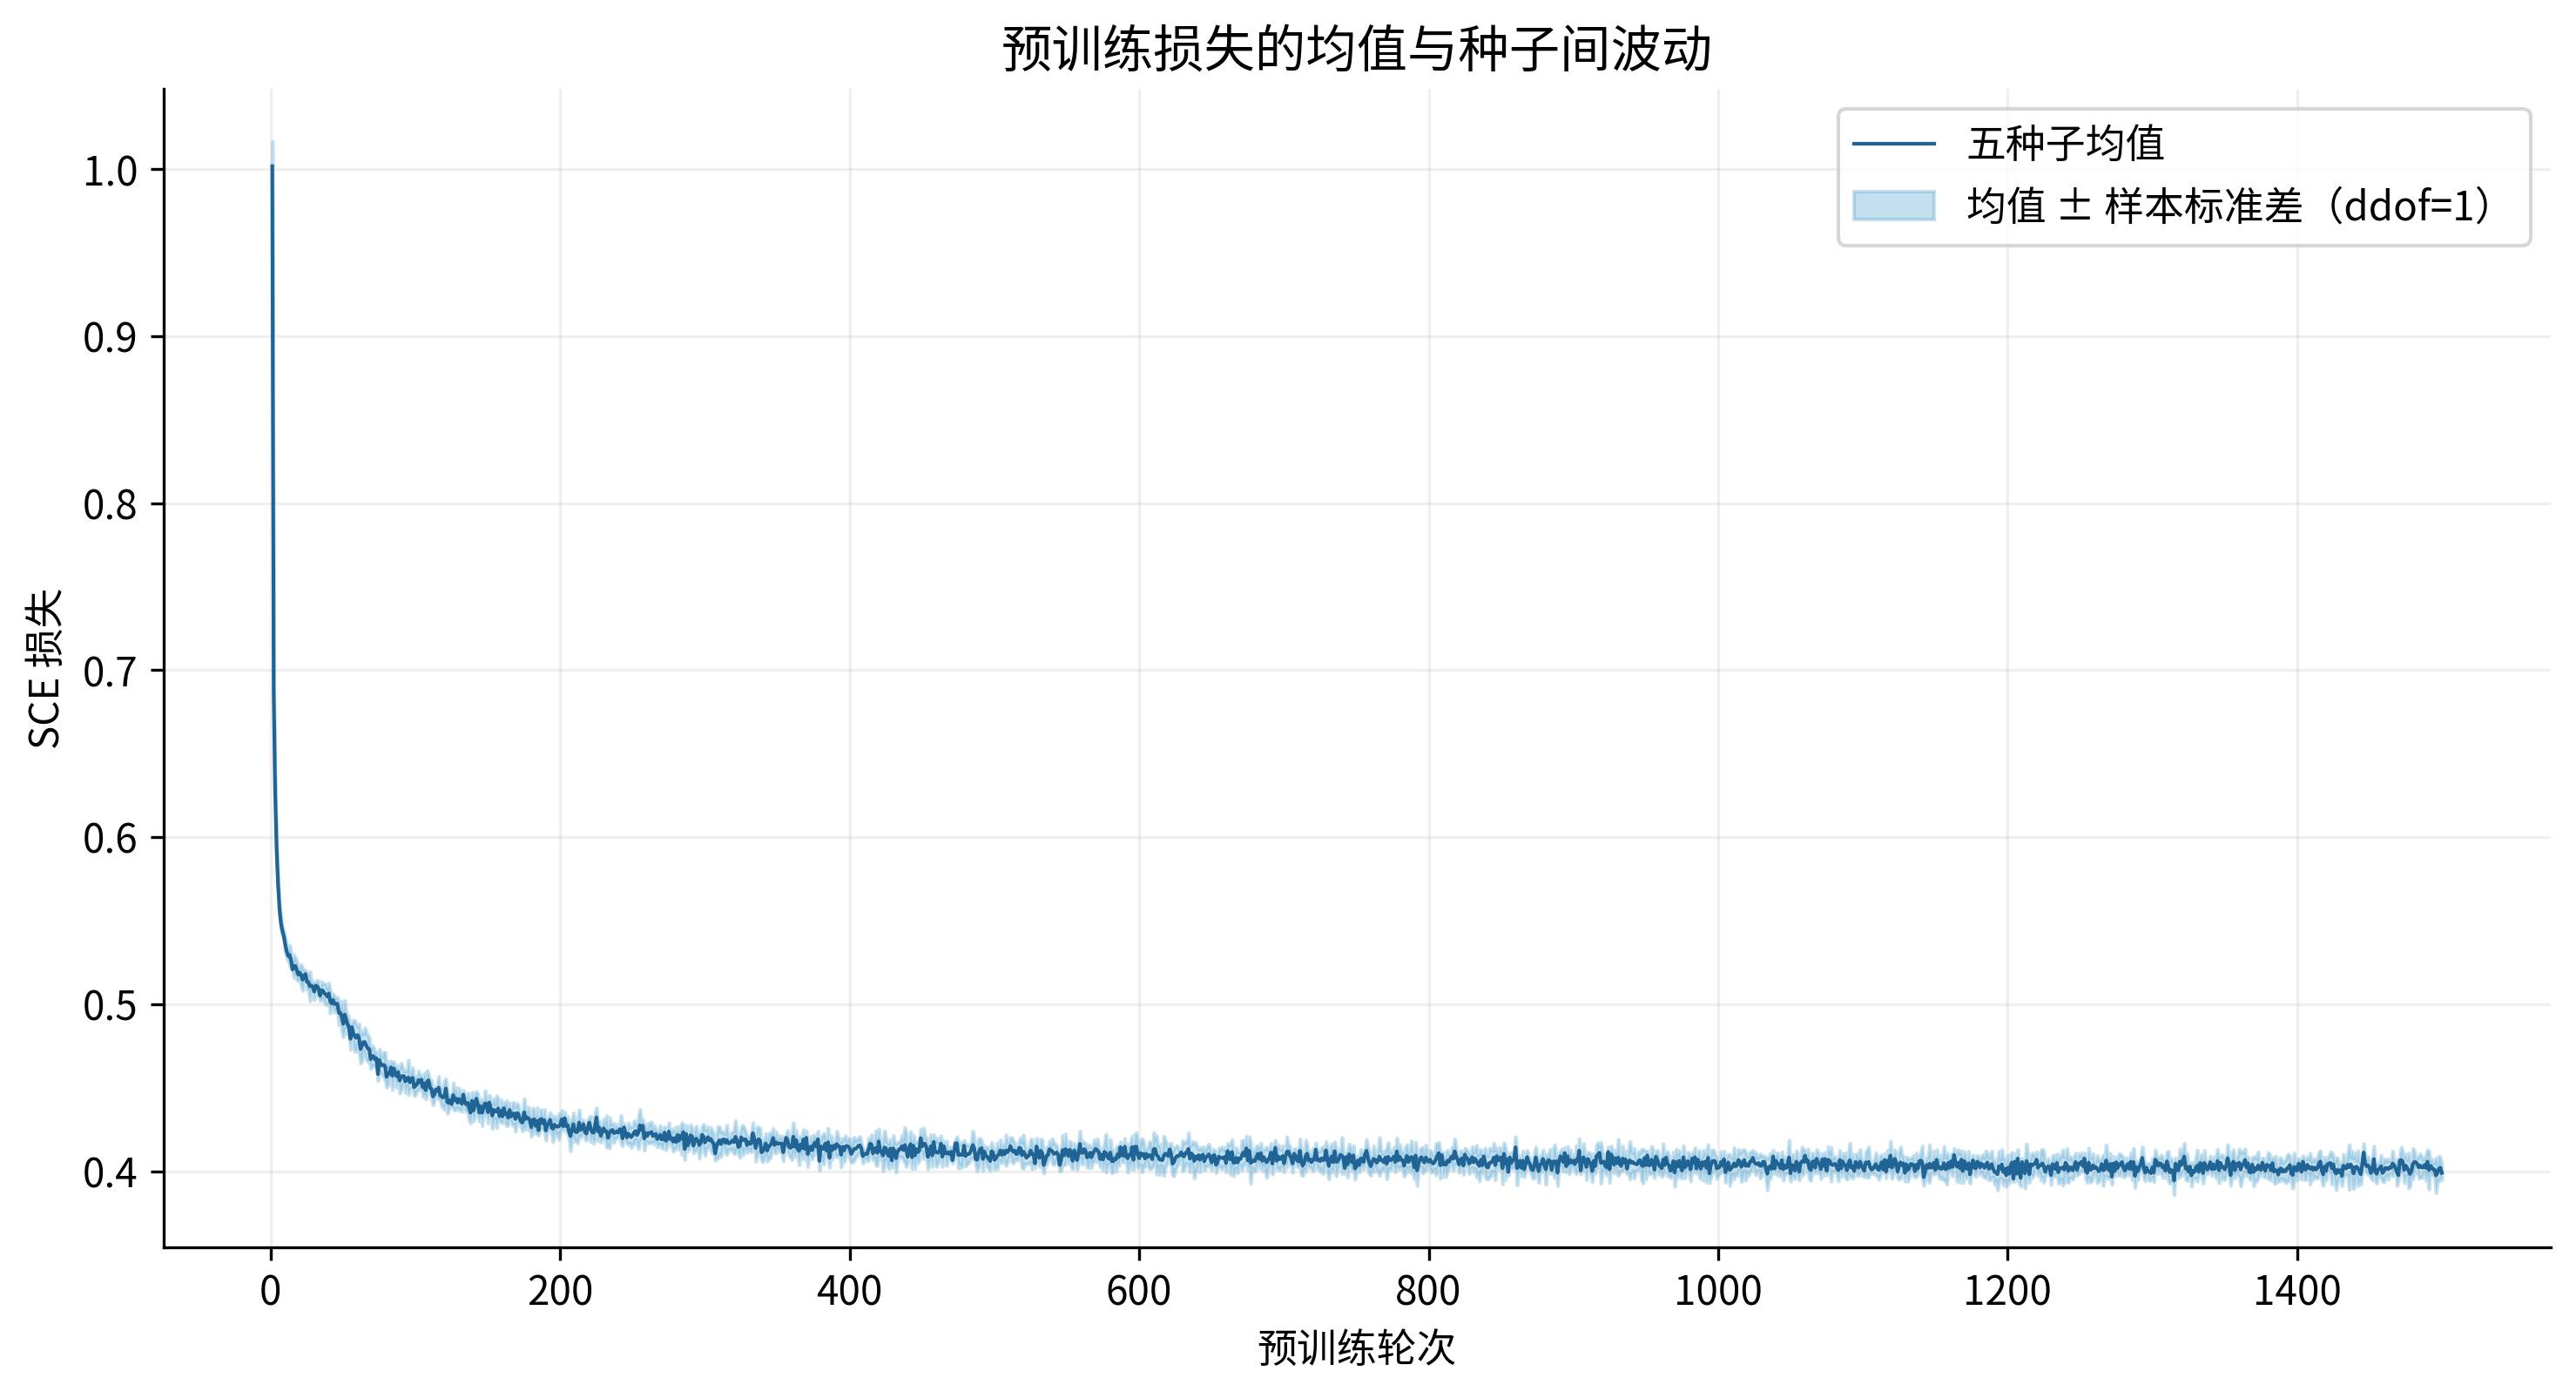
\includegraphics[width=0.86\linewidth]{../figures/M1/loss_mean_std.png}
\caption{M1五种子的预训练SCE均值与波动带。阴影为逐轮跨种子的样本标准差，来源为各次1500轮训练日志；未包含M0短测。}\label{fig:m1-loss}
\end{figure}

\subsection{与原论文结果的参考性比较}
M1测试均值为83.98\%，样本标准差为1.056882个百分点。原论文表1的Cora结果为$84.2\%\pm0.4\%$，采用20次初始化；本项目均值低0.22个百分点。图\ref{fig:m1-accuracy}仅以论文均值提供参考，不代表二者采用完全相同的重复次数和运行环境。
\begin{figure}[tbp]
\centering
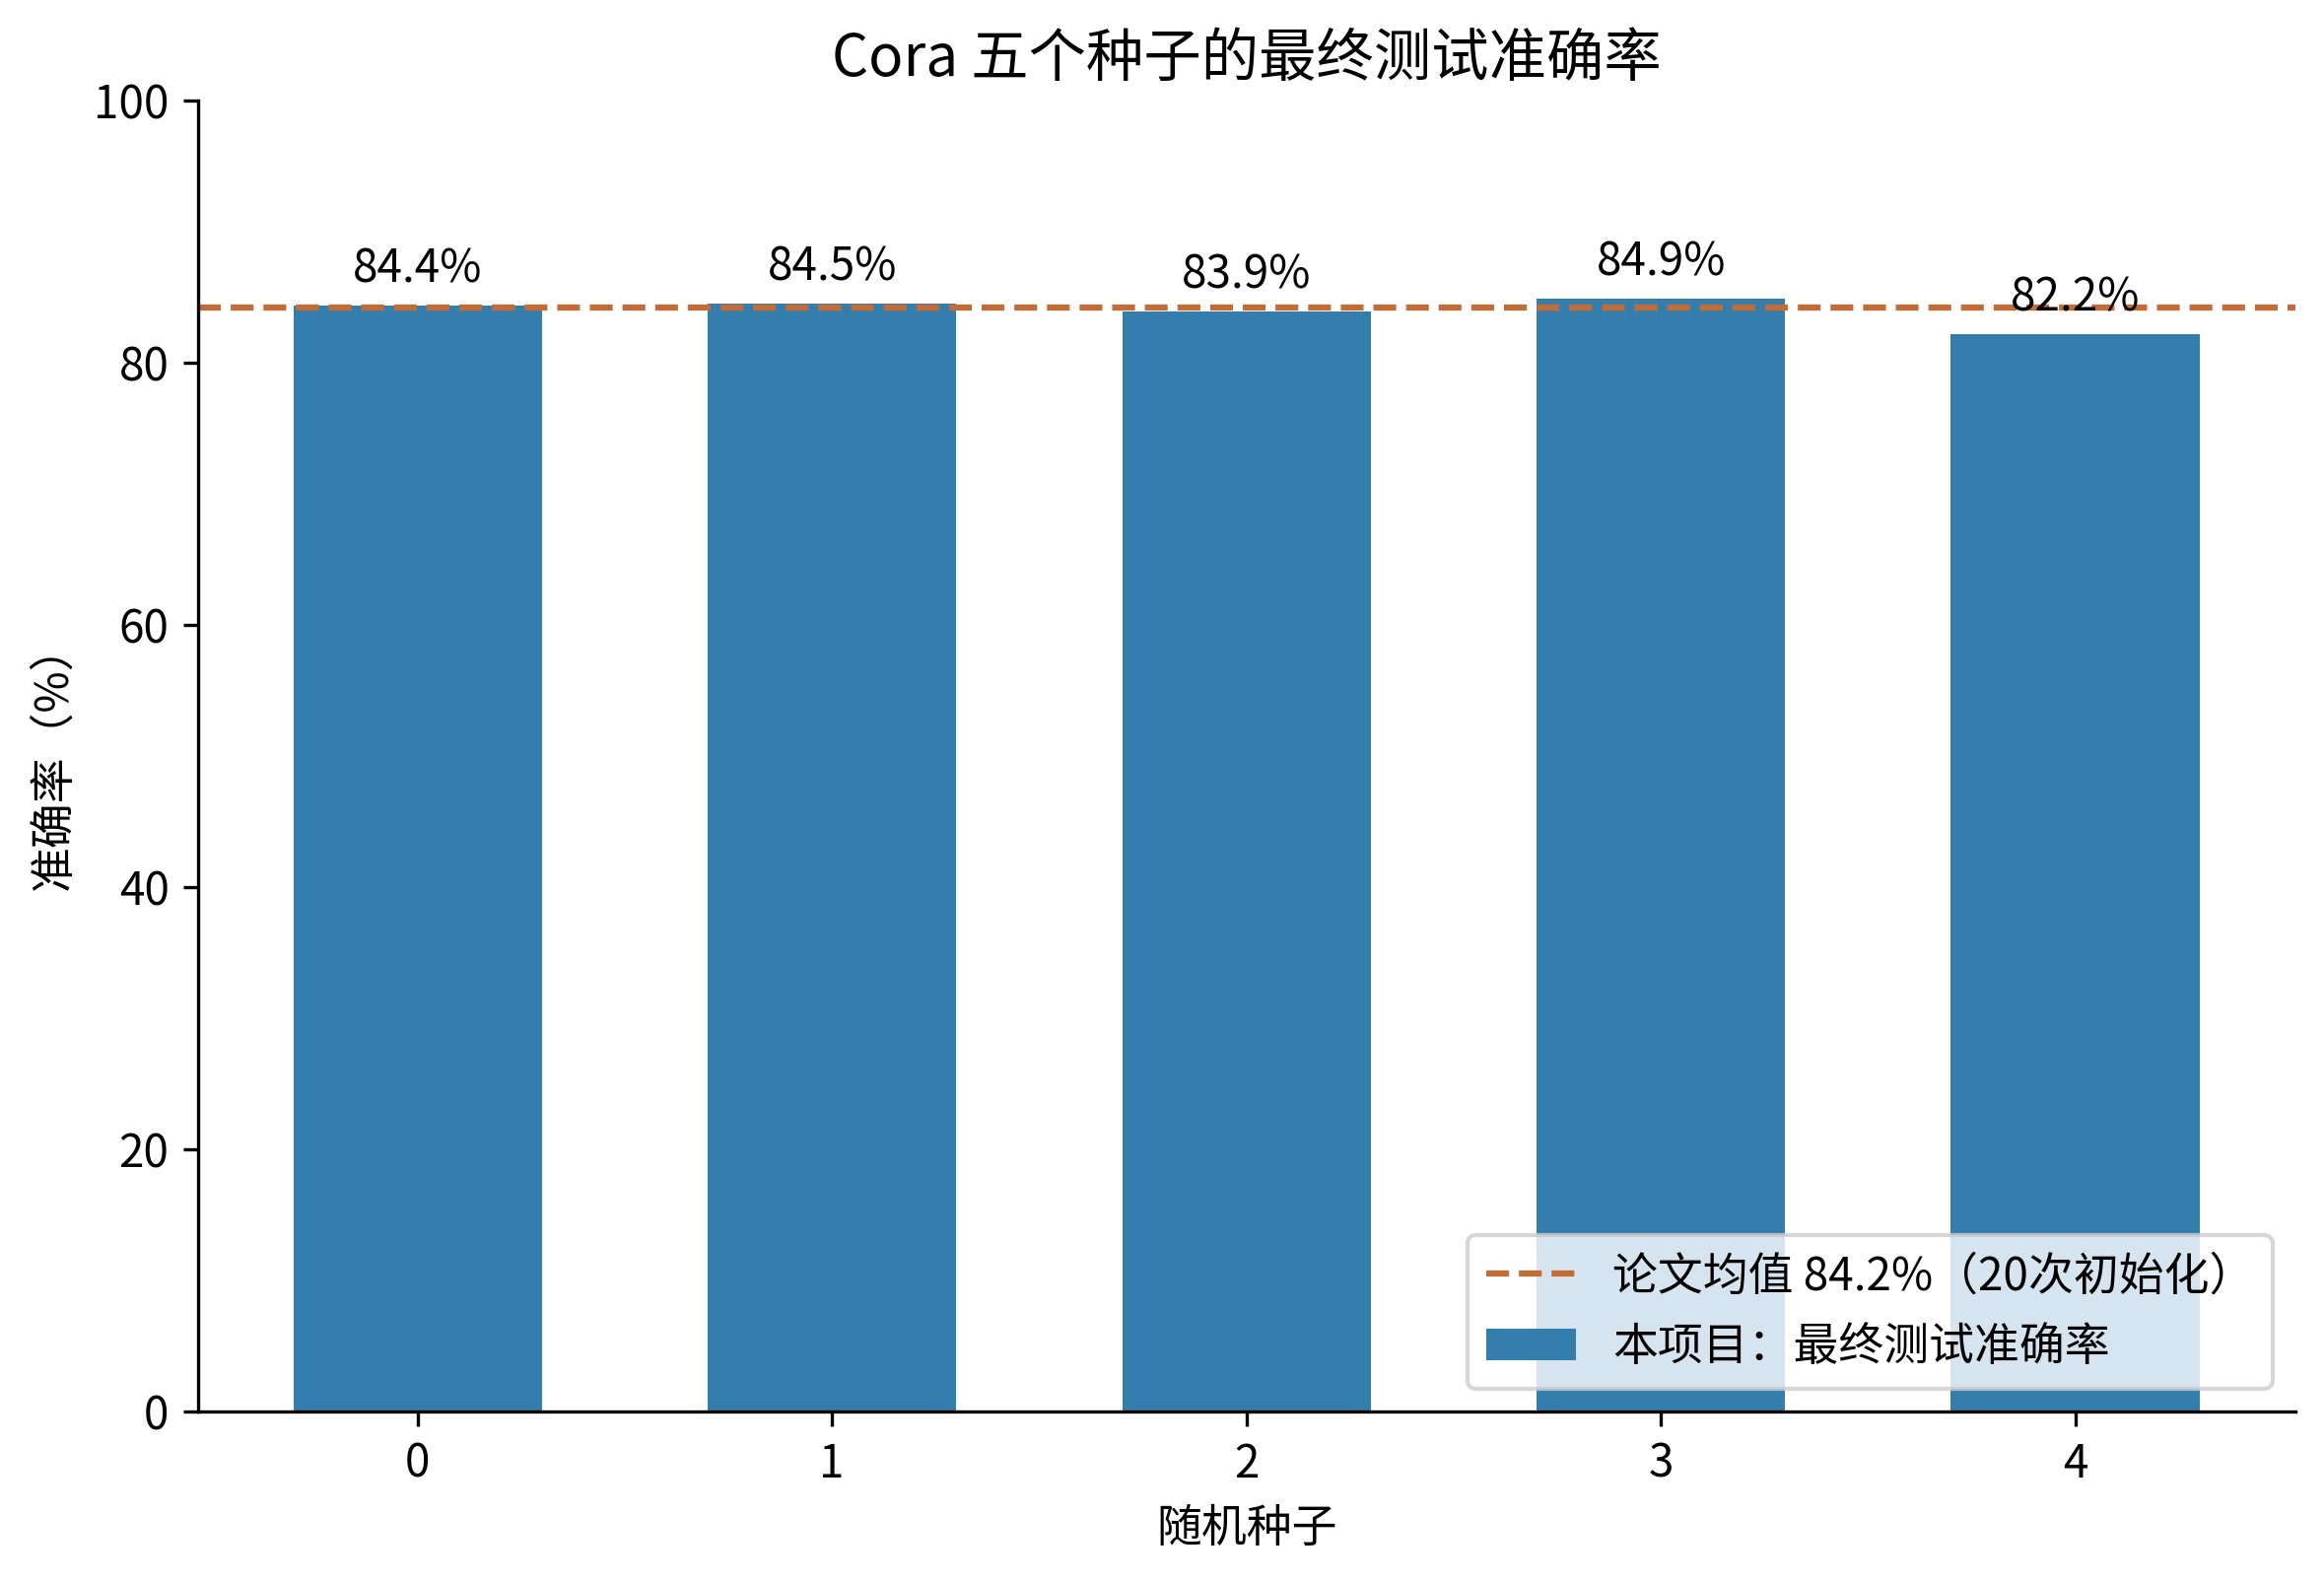
\includegraphics[width=0.86\linewidth]{../figures/M1/accuracy_comparison.png}
\caption{M1五种子的最终测试准确率。虚线为原论文20次初始化的均值84.2\%\cite{hou2022graphmae}；五个柱为本地实测，不能将论文参考线当成本地额外实验。}\label{fig:m1-accuracy}
\end{figure}

五种子的最高与最低准确率为84.9\%和82.2\%，范围为2.7个百分点。seed4虽使总体波动增大，仍按预设种子完整保留，没有重训或剔除。验证最优轮次差异也提示，在只有140个训练标签时，分类器选择对初始化与表示差异较敏感；这是一种现象描述，不足以确定波动来自哪个模型组件。

本次采用PyG、PyTorch 2.4.1和A40，原论文主要使用DGL、PyTorch 1.9和2080Ti。本文使用样本SD，官方代码汇总中\texttt{np.std}默认采用总体SD；原论文未明确给出其标准差实现细节，不能把二者强行视为同一统计口径。此外，本项目仅完成Cora的五次初始化，并未复现其他任务。因此，结果说明锁定官方路径获得了接近论文报告量级的分类表现，同时保留了较大种子波动；不能据均值接近宣称完整复现。

\section{Degree-aware Masking方法设计}\label{sec:degree-method}
\subsection{动机与度数定义}
均匀策略使每个节点每轮具有相同纳入概率，不考虑可用于重建的邻域大小。本文提出一个探索性假设：高度数节点具有更多邻居上下文，适度提高其被掩码频率，或可促使编码器学习这部分节点的表示。然而，高度数节点也影响更多邻居，同时遮蔽它们可能削弱上下文，低度数节点获得的重建监督则可能减少。该假设需要通过实验判断，不预设正向效果。

从与M1相同的预处理图中排除所有自环，并以唯一邻居定义度数：
\begin{equation}\label{eq:degree}
d_i=\left|\{j\ne i:\{i,j\}\in E_{\rm unique}\}\right|,
\qquad w_i=(d_i+1)^{\alpha_d}.
\end{equation}
$E_{\rm unique}$表示去重后的无向邻居关系，$w_i>0$为采样权重。当前Cora非自环条目已经双向对称且没有重复；仍保留唯一邻居核查，防止边重复造成度数偏大。度数向量只计算一次，全部实验共用，计算和分组都不使用标签。参数$\alpha_d$在代码中命名为\texttt{degree\_alpha}，与SCE的$\gamma=\texttt{alpha\_l}=3$分别控制不同机制。

\subsection{固定预算的加权无放回采样}
当$\alpha_d>0$时，权重随度数增大；$\alpha_d$越大，相同度数差异对应的相对权重差越明显。实际采样为
\begin{equation}\label{eq:weighted-mask}
M\sim\operatorname{WeightedWithoutReplacement}(w,k),\qquad
k=\lfloor0.5\times2708\rfloor=1354.
\end{equation}
正向方案使用\texttt{torch.multinomial}、\texttt{replacement=False}及独立CPU随机生成器；每轮选点无重复。权重是抽样输入，而$\Pr(i\in M)$是固定预算下的最终边际纳入概率，二者不能简单写成$w_i/\sum_jw_j$。实际分布通过逐节点掩码次数核验。

图\ref{fig:degree-flow}给出策略的信息流。除了选点分布，mask token、随机特征替换、Re-mask、模型结构及SCE均保持不变，也没有加重要性校正。因此它会改变各类节点对预训练目标的期望贡献，而非只改变等价目标的实现速度。
\begin{figure}[tbp]
\centering
% Editable TikZ source; included by main.tex, not a standalone document.
\begin{tikzpicture}[
  node distance=5mm and 5mm,
  box/.style={draw,rounded corners=2pt,align=center,minimum height=12mm,
    text width=25mm,inner sep=3pt,font=\small},
  flow/.style={-{Latex[length=2mm]},thick}]
\node[box] (graph) {图结构\\去自环、去重};
\node[box,right=of graph] (degree) {唯一邻居度数\\$d_i=|\mathcal N(i)|$};
\node[box,right=of degree] (weight) {掩码权重\\$(d_i+1)^{\alpha_d}$};
\node[box,right=of weight] (sample) {无放回采样\\$|M|=1354$};
\node[box,below=7mm of sample] (train) {原GraphMAE\\重建训练};
\draw[flow] (graph)--(degree);
\draw[flow] (degree)--(weight);
\draw[flow] (weight)--(sample);
\draw[flow] (sample)--(train);
\node[align=left,font=\small,anchor=east,left=5mm of train] {只调整节点选择分布\\模型、掩码预算与损失保持不变};
\end{tikzpicture}

\caption{本文度数感知掩码策略的流程示意。图中仅显示方法定义，不包含虚构的实验取样结果。均匀控制组仍使用randperm，正向方案使用加权无放回采样。}\label{fig:degree-flow}
\end{figure}

\subsection{实验分组与随机数流控制}
四组参数为$\alpha_d=0,0.25,0.5,1.0$，每组使用种子0--4，共20次正式训练。$\alpha_d=0$的控制组仍采用均匀randperm，未将multinomial用作控制组算法。所有组均完整执行表\ref{tab:hyperparameters}的训练预算。正式实验前四个seed0短程Pilot各训练20轮预训练和20轮Probe，不评价测试集，也不计入正式统计。

不同采样函数可能消耗不同数量的随机数，进而改变Dropout等后续操作。为减少该混杂，M2把实际选点放到独立CPU \texttt{torch.Generator(seed)}：控制组使用CPU randperm，正向组使用CPU double权重的multinomial。四组在实际选点前都调用并丢弃一次与官方同设备、同形状的\texttt{randperm(N)}结果，随后沿用原有\texttt{randperm(k)}分配token/替换节点，以及\texttt{randperm(N)}选择特征供体。这样，策略分支的额外随机消耗不进入模型初始化、替换和Dropout的全局随机流。

实际检查确认同seed四组的初始模型权重哈希一致，短程GPU诊断中的替换顺序与6次Dropout调用状态一致，正式1500轮的CPU/CUDA全局RNG和替换轨迹逐行一致。但这并不消除GPU浮点归约非确定性。由于M1实际选点使用全局CUDA randperm，M2独立CPU选点的均匀控制组必须重新训练，不能直接拿M1的83.98\%作为本章对照；M2内部四组才使用同一随机协议。

\section{自主实验结果与分析}\label{sec:m2-results}
\subsection{验证集结果与正向系数选择}
四组共20次训练及所有Probe均完整完成，训练和验证损失没有NaN或Inf。表\ref{tab:m2-validation}及图\ref{fig:m2-validation}显示，各正向系数的验证均值均低于均匀控制组，且在本次三个候选值上随系数增大而下降。

令$v_{\alpha,s}=\max_t\operatorname{Acc}_{\rm val}^{(\alpha,s)}(t)$为固定第1500轮encoder对应最终Probe的最佳验证准确率。预设的正向参数选择规则为
\begin{equation}\label{eq:alpha-selection}
\bar v_\alpha=\frac15\sum_{s=0}^{4}v_{\alpha,s},\qquad
\alpha_d^*=\min\arg\max_{\alpha\in\{0.25,0.5,1.0\}}\bar v_\alpha.
\end{equation}
实际用验证正确数的整数总和比较，避免浮点平分歧义。控制组不在“最佳正向系数”候选集合内，所以即使所有正向方案较差，仍保留其中最佳的0.25进行预定比较。它的验证均值比控制组低0.44个百分点，不能描述为验证阶段胜出控制组。

选择记录于2026年11月14日07:27:47 UTC封存，记录全部20次结果与checkpoint哈希，早于最终测试启动。封存后仅测试控制组与0.25各五个模型，每个模型一次；0.5和1.0没有最终测试。训练阶段的周期与最终Probe仅使用训练、验证标签。
\begin{table}[tbp]
\centering\small
\caption{M2四组五种子的验证结果与最终测试适用性。均值单位为\%，SD单位为百分点；测试列未用于式\eqref{eq:alpha-selection}。}\label{tab:m2-validation}
\begin{tabular}{lrrrr}\toprule
$\alpha_d$ & 验证均值 & 验证样本SD & 测试均值 & 测试样本SD\\\midrule
0（控制） & 80.04 & 0.2191 & 84.20 & 0.3674\\
0.25 & 79.60 & 0.7616 & 82.92 & 1.6664\\
0.5 & 78.52 & 0.4817 & \multicolumn{2}{c}{未测试}\\
1.0 & 76.16 & 2.2064 & \multicolumn{2}{c}{未测试}\\\bottomrule
\end{tabular}
\end{table}
\begin{figure}[tbp]
\centering
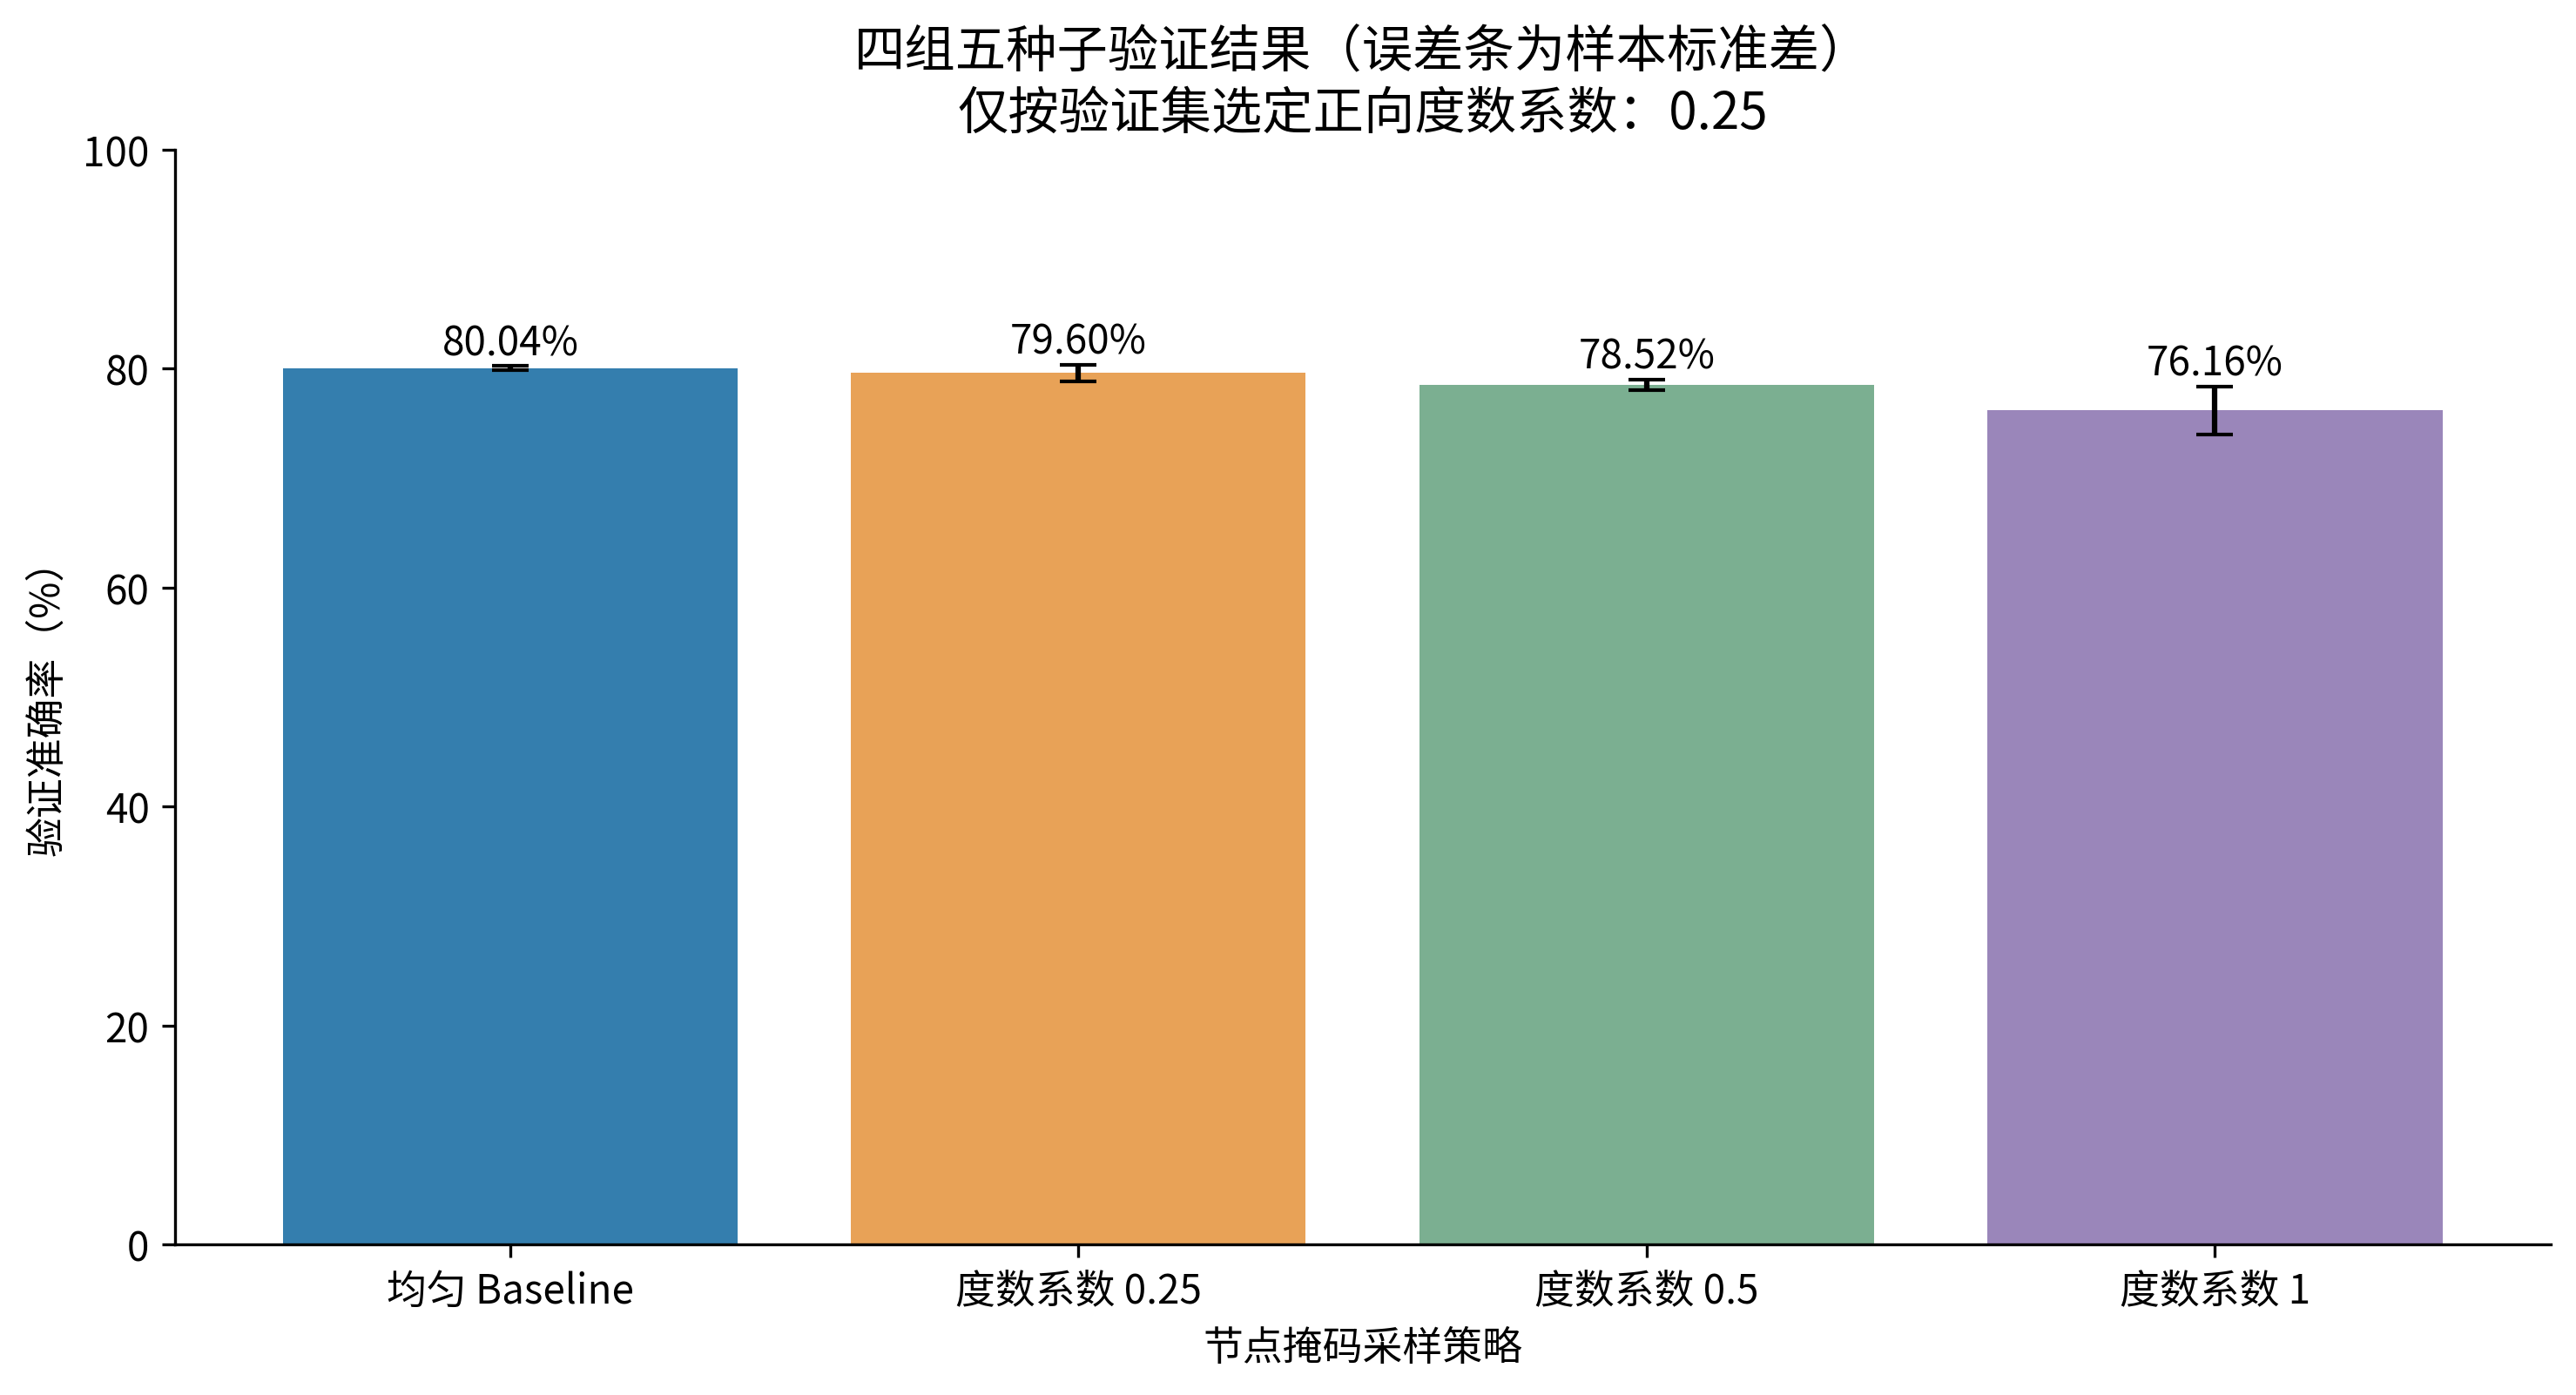
\includegraphics[width=0.88\linewidth]{../figures/M2/validation_comparison.png}
\caption{四组最终Probe最佳验证准确率的五种子均值及样本SD。0.25只在预设正向系数中最好，全部正向方案均低于控制组。}\label{fig:m2-validation}
\end{figure}

\subsection{最终测试与逐种子配对比较}
表\ref{tab:m2-paired}和图\ref{fig:m2-paired}保留五个种子的一一配对结果。定义每对变化为
\begin{equation}\label{eq:paired}
\Delta_s=100\left(a_{0.25,s}-a_{0,s}\right)\quad\text{（百分点）},
\end{equation}
其中$a$取0--1比例。控制组测试均值为84.20\%，样本SD为0.367423个百分点；0.25为82.92\%，样本SD为1.666433个百分点。平均配对变化为$-1.28$个百分点，配对差值的样本SD为1.682855个百分点。后者由五个差值计算，不是简单将两组SD相减。
\begin{table}[tbp]
\centering\small
\caption{M2最终测试的五种子配对。Accuracy单位为\%，差值单位为百分点。}\label{tab:m2-paired}
\begin{tabular}{rrrr}\toprule
Seed & 均匀控制组 & Degree-aware 0.25 & $\Delta_s$\\\midrule
0 & 84.20 & 80.10 & $-4.10$\\
1 & 84.80 & 83.50 & $-1.30$\\
2 & 84.10 & 84.00 & $-0.10$\\
3 & 84.10 & 84.20 & $+0.10$\\
4 & 83.80 & 82.80 & $-1.00$\\\midrule
均值 & 84.20 & 82.92 & $-1.28$\\
样本SD & 0.37 & 1.67 & 1.68\\\bottomrule
\end{tabular}
\end{table}
\begin{figure}[tbp]
\centering
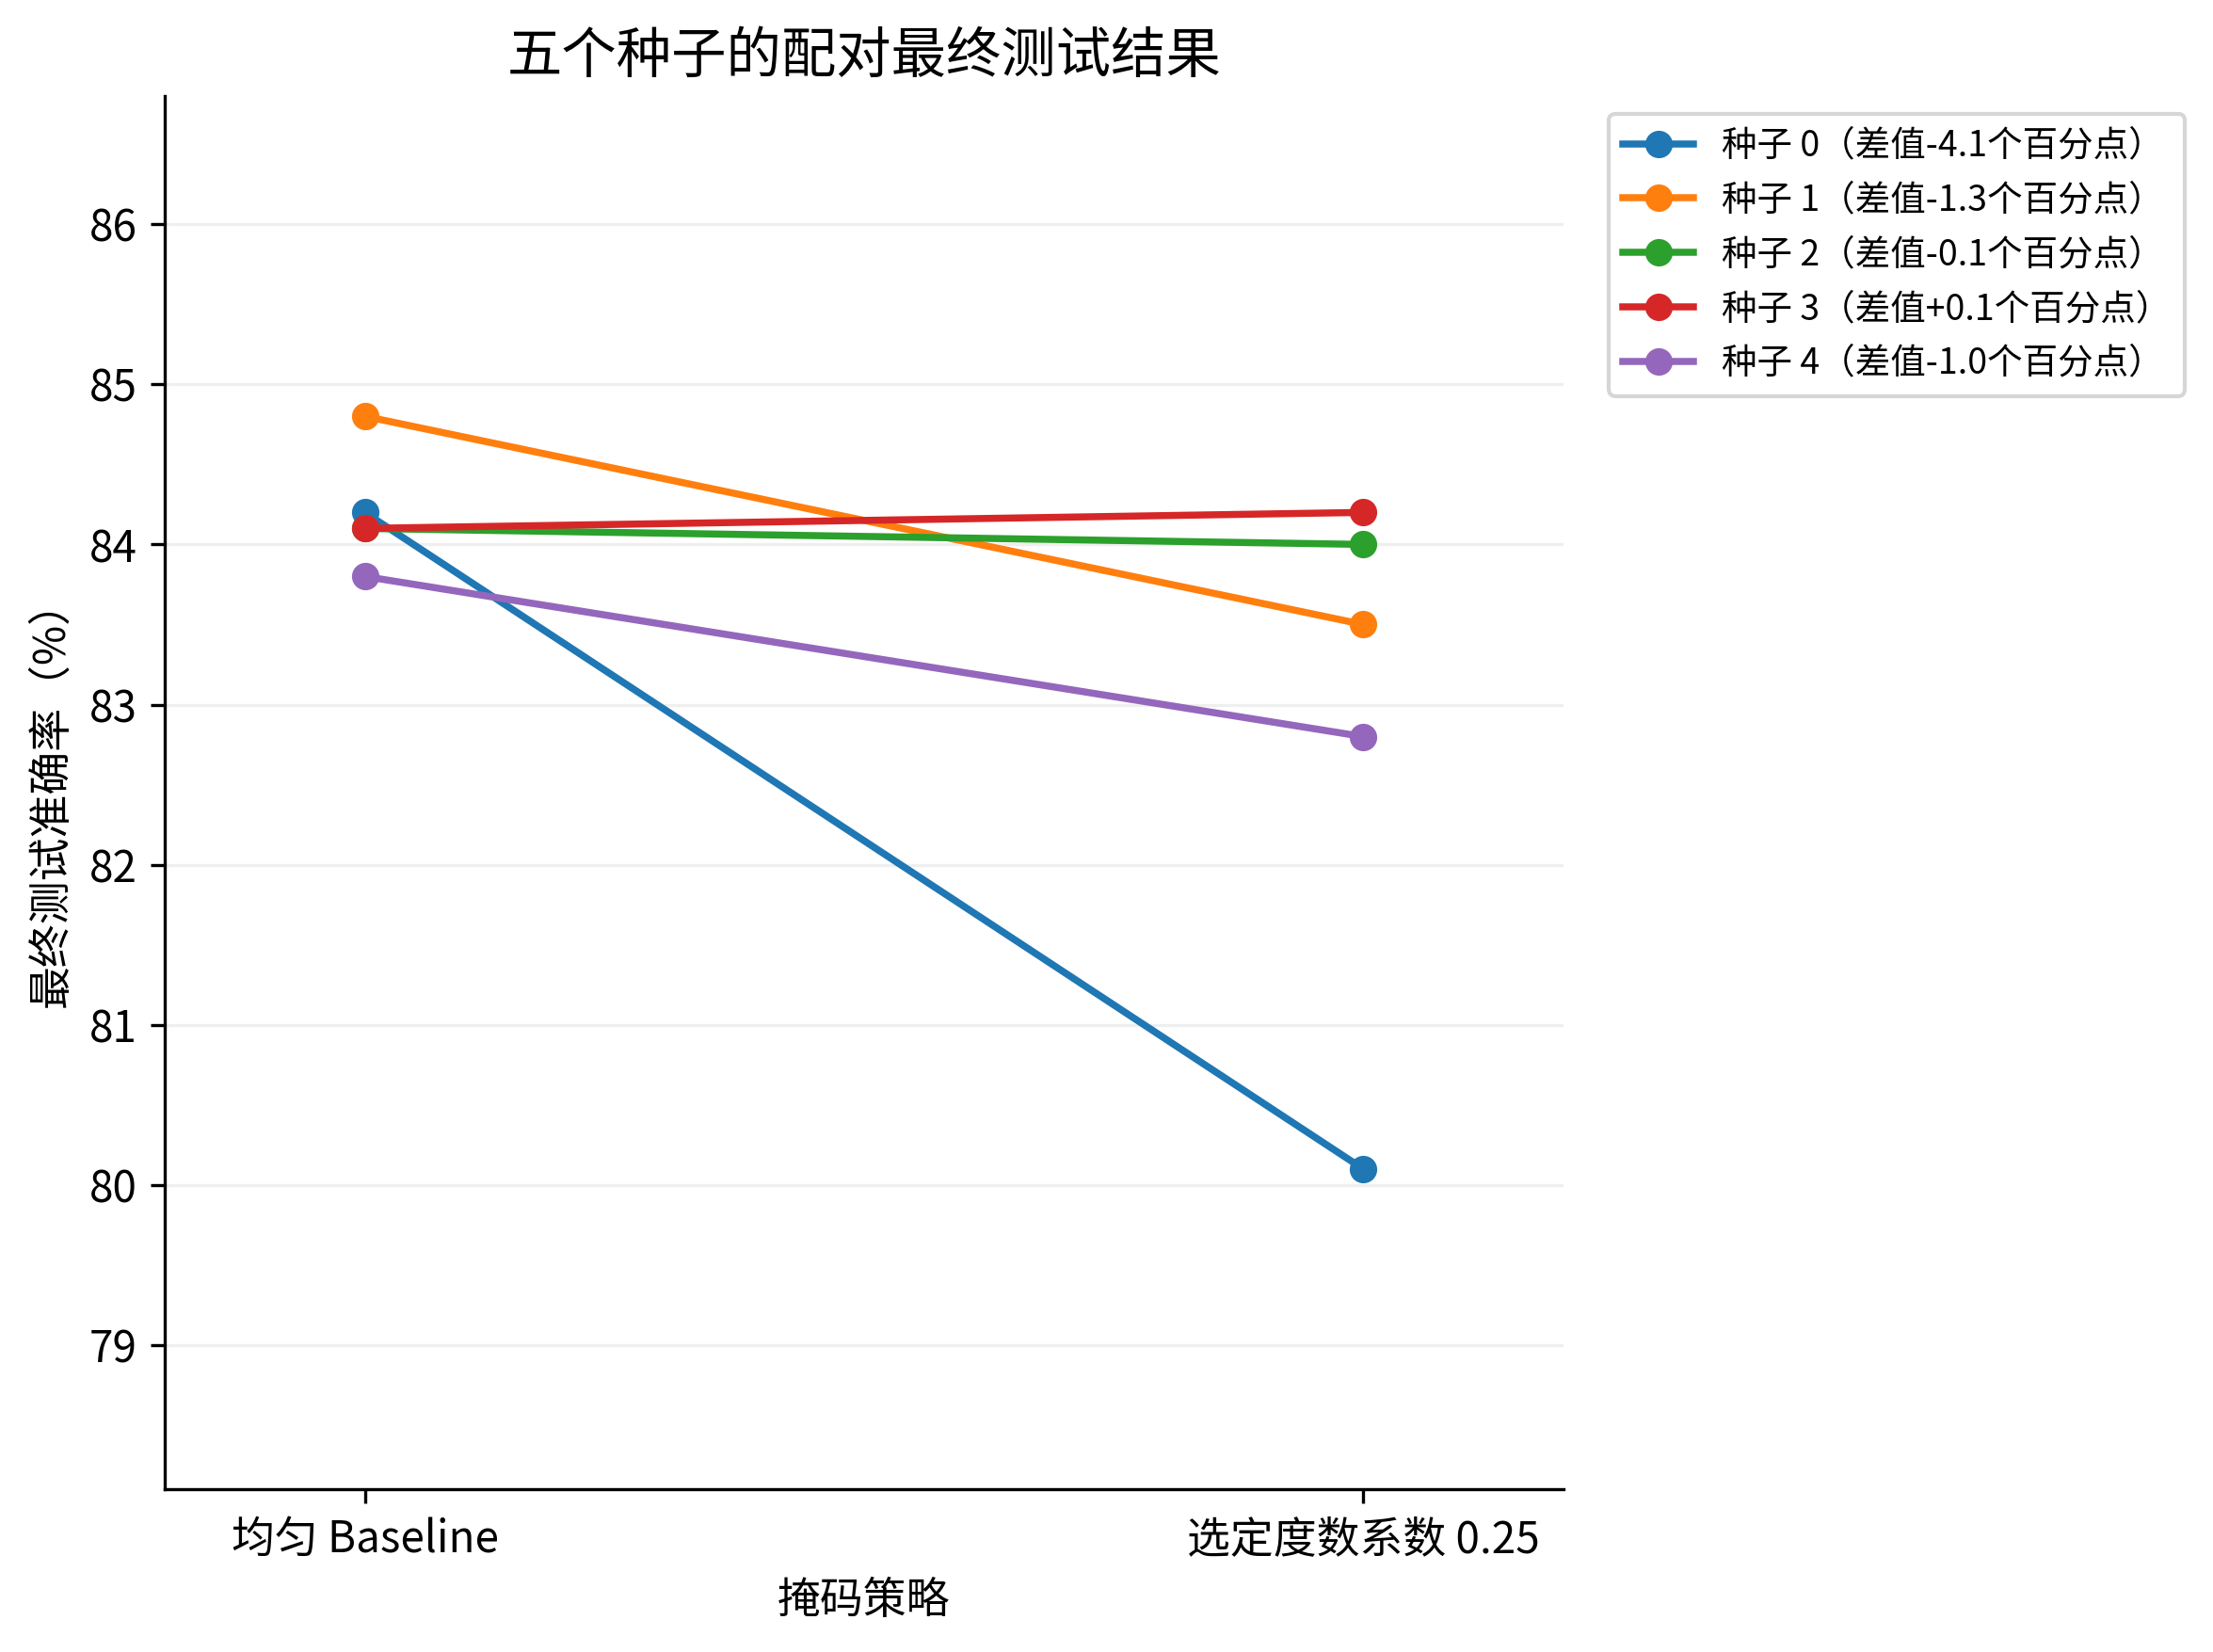
\includegraphics[width=0.88\linewidth]{../figures/M2/paired_test_accuracy.png}
\caption{控制组与0.25方案的逐种子配对测试结果。每条线对应同一seed，纵轴采用局部范围以展示差异，全部五对均保留。}\label{fig:m2-paired}
\end{figure}

五对中四对下降，一对提高0.10个百分点；seed0下降4.10个百分点，是本次波动的重要组成部分。不能仅展示seed3的小幅提高，也不能因seed0不利而重训或删除。该结果未支持本次配置下的平均性能改善假设，但仅五对重复不足以据此作普遍性结论或充分的统计推断。

\subsection{度数感知掩码是否真正生效}
全图度数最小为1、最大为168、均值3.898080、中位数3。分组边界在训练前仅按结构确定：在不拆分同度数节点的条件下，选择使三组人数相对$N/3$平方偏差之和最小的两个边界，得到低度数1--2、中度数3--4、高度数5--168，人数分别为1068、942、698。因此这些组不是严格等人数的三分位。

设$V_g$为度数组$g$的节点集合，$c_i$为节点$i$在1500轮中被选中的次数。组内实际掩码率为
\begin{equation}\label{eq:mask-rate}
c_i=\sum_{t=1}^{1500}\mathbf1\{i\in M_t\},\quad
\widehat r_g=\frac{\sum_{i\in V_g}c_i}{1500|V_g|},\quad
\overline c_g=\frac{\sum_{i\in V_g}c_i}{|V_g|}.
\end{equation}
它回答“该组一个节点在一轮中平均多常被掩码”，不同于该组占全部掩码选择的份额，后者分母为$1500\times1354$。

图\ref{fig:m2-mask}显示均匀控制组各组掩码率均接近50\%；0.25时低、中、高度数组分别约为45.68\%、50.52\%、55.90\%。对应平均被选次数为685.27、757.84、838.47，而控制组约为750.01、749.65、750.46。系数进一步增大至0.5和1.0时，高度数组掩码率达到61.67\%和71.98\%，低度数组降为41.56\%和34.14\%。每轮总选点始终为1354，故这种偏移不是由额外增加训练目标数量造成。实际频率说明度数权重确实改变了采样分布，实现生效与分类收益应分别判断。
\begin{figure}[tbp]
\centering
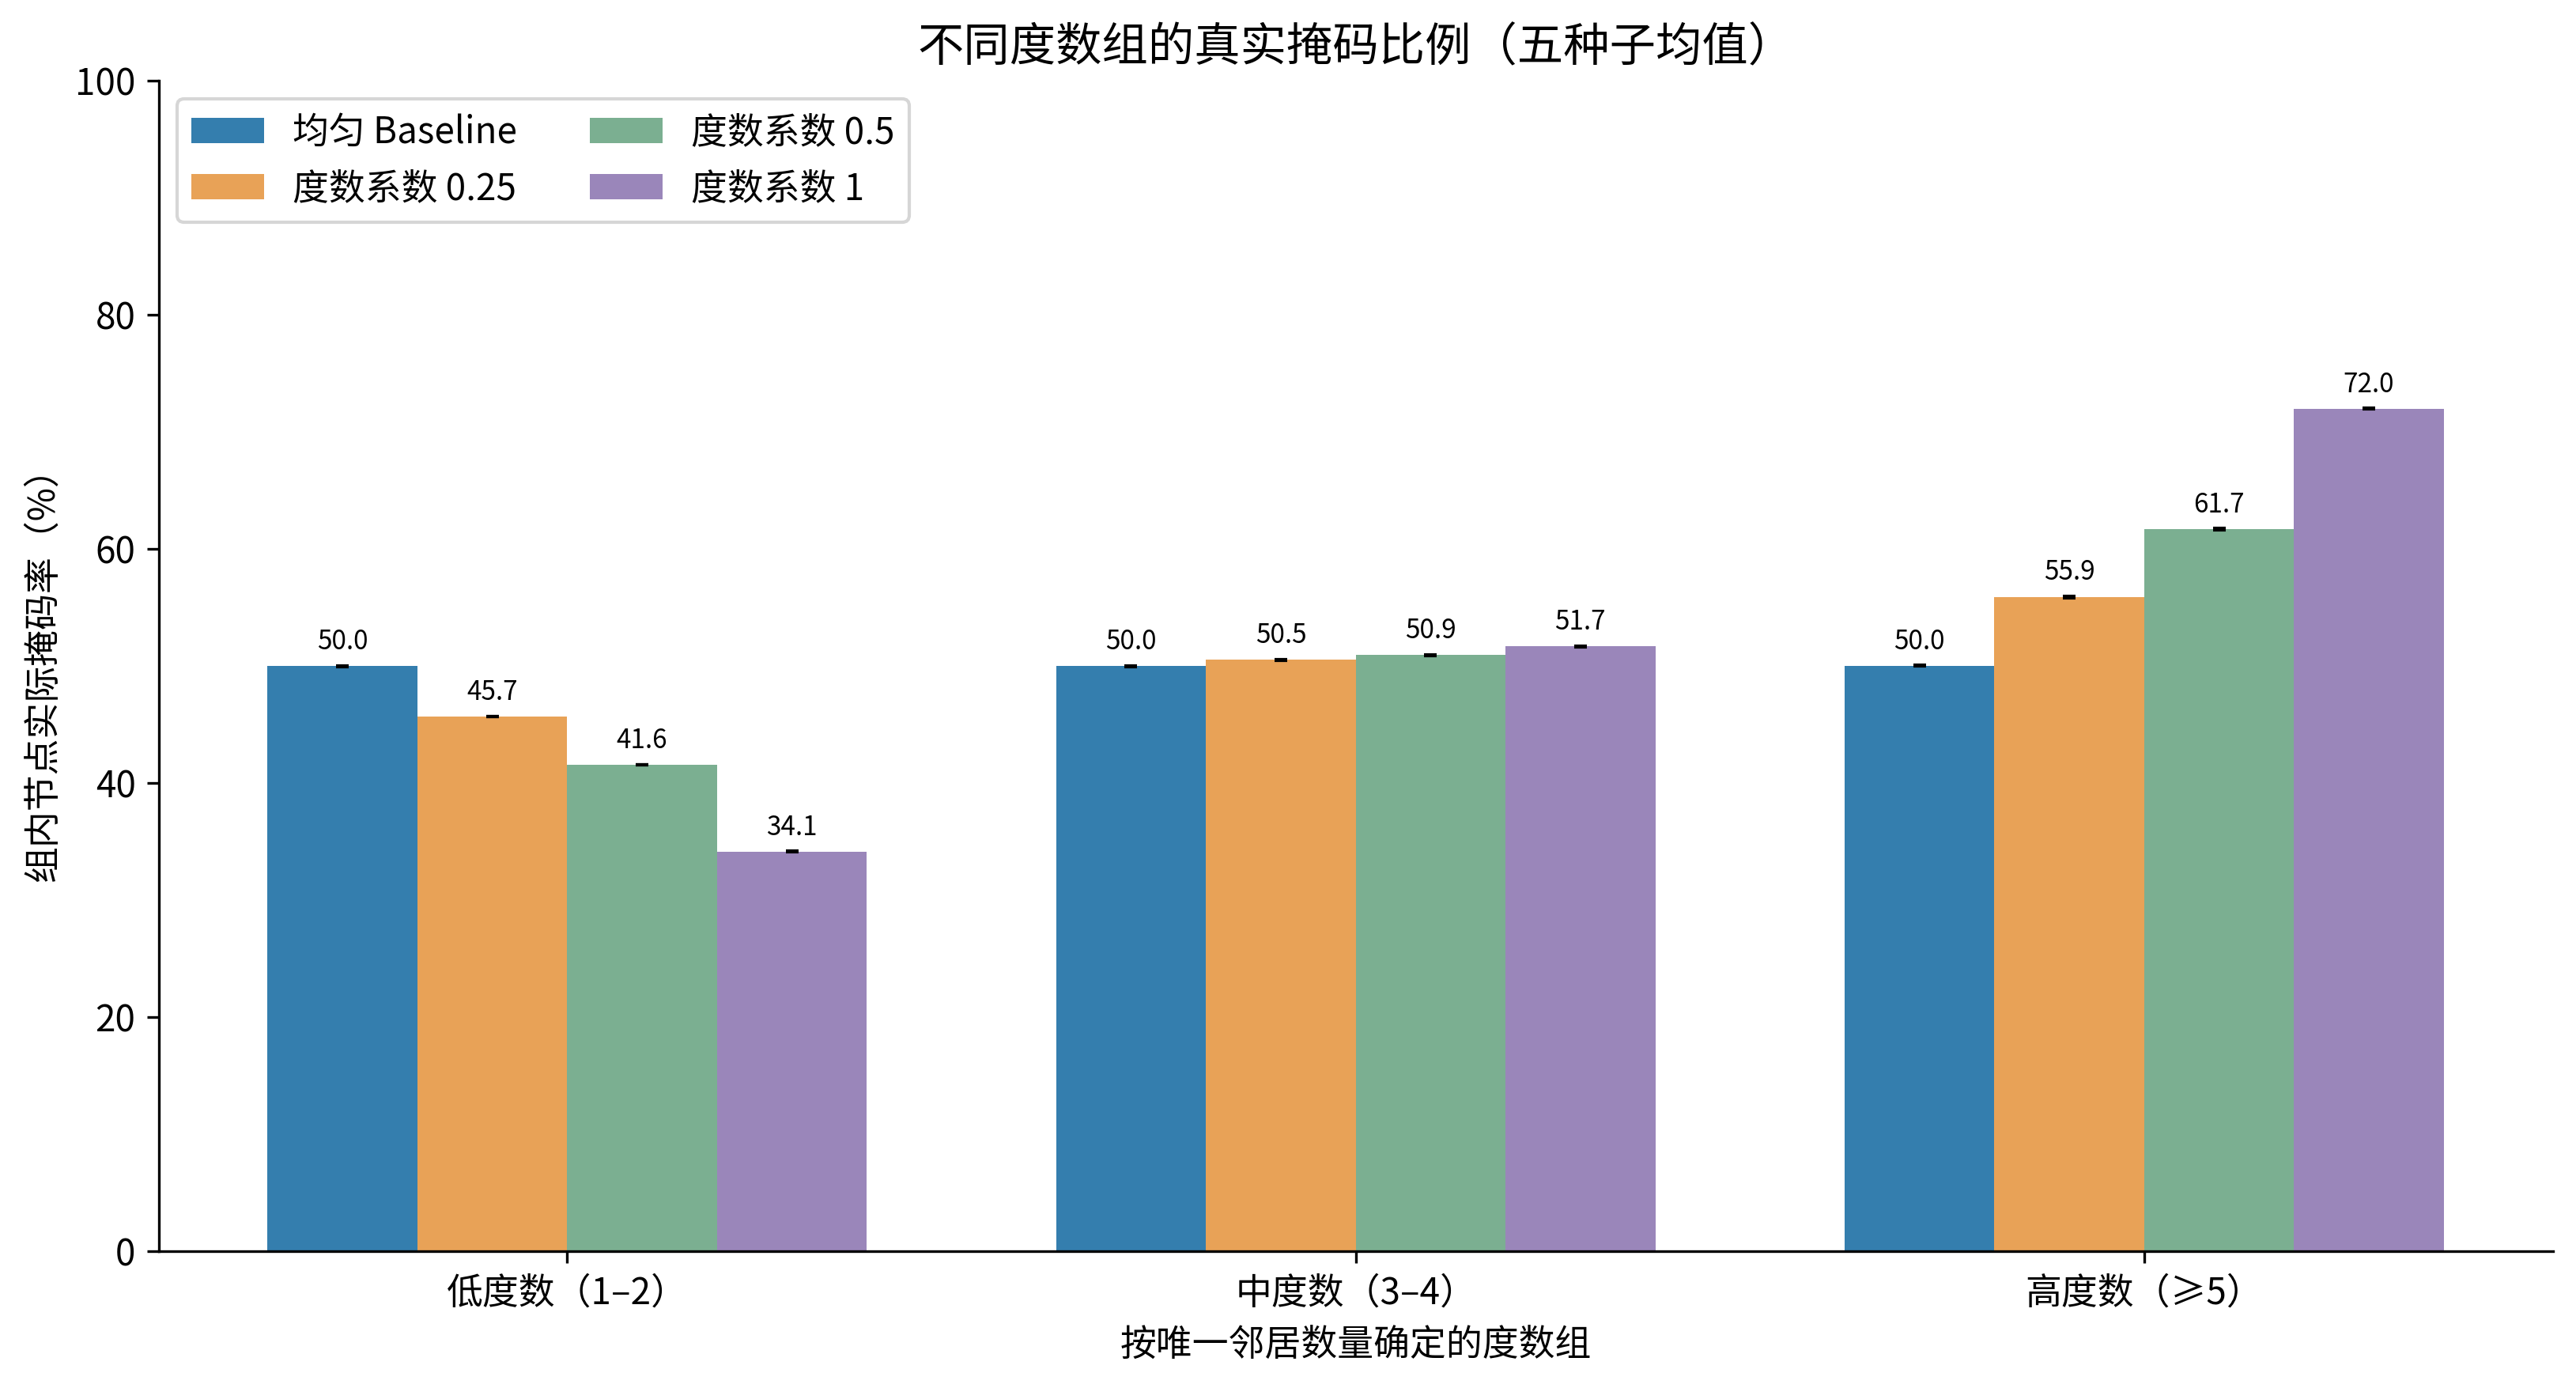
\includegraphics[width=0.92\linewidth]{../figures/M2/degree_mask_rates.png}
\caption{各度数组的组内实际掩码率，使用每次1500轮的逐节点计数汇总。柱为五种子均值，误差条为样本SD；所有组均固定每轮1354个节点。}\label{fig:m2-mask}
\end{figure}

\subsection{不同度数组的分类表现}
最终参数封存后，使用同一次测试保存的预测计算分组准确率，没有再次运行模型或依分组测试结果重选系数。对于组$g$，
\begin{equation}\label{eq:group-accuracy}
\operatorname{Acc}_g=\frac{\sum_{i\in V_g\cap V_{\rm te}}\mathbf1\{\widehat y_i=y_i\}}
{|V_g\cap V_{\rm te}|}.
\end{equation}
表\ref{tab:degree-groups}和图\ref{fig:m2-groups}显示三组平均均下降，低、中、高组分别下降0.95、约1.38、约1.67个百分点。高度数组虽增加了掩码监督，却没有取得预期的平均分类收益。中度数组Accuracy高于低度数组是当前节点集合上的观察，不能解释为度数增大必然提升分类。
\begin{table}[tbp]
\centering\small
\caption{度数组规模与最终测试结果。正确数为同一测试划分的五次预测合计；Accuracy为五种子均值，不把重复评价次数当独立节点数。}\label{tab:degree-groups}
\footnotesize
\setlength{\tabcolsep}{4pt}
\begin{tabular}{lrrrrr}\toprule
度数组 & 全图人数 & 测试人数/seed & 控制正确数 & 0.25正确数 & Accuracy：控制/0.25\\\midrule
低：1--2 & 1068 & 400 & 1575/2000 & 1556/2000 & 78.75/77.80\%\\
中：3--4 & 942 & 348 & 1543/1740 & 1519/1740 & 88.68/87.30\%\\
高：5--168 & 698 & 252 & 1092/1260 & 1071/1260 & 86.67/85.00\%\\\bottomrule
\end{tabular}
\end{table}
\begin{figure}[tbp]
\centering
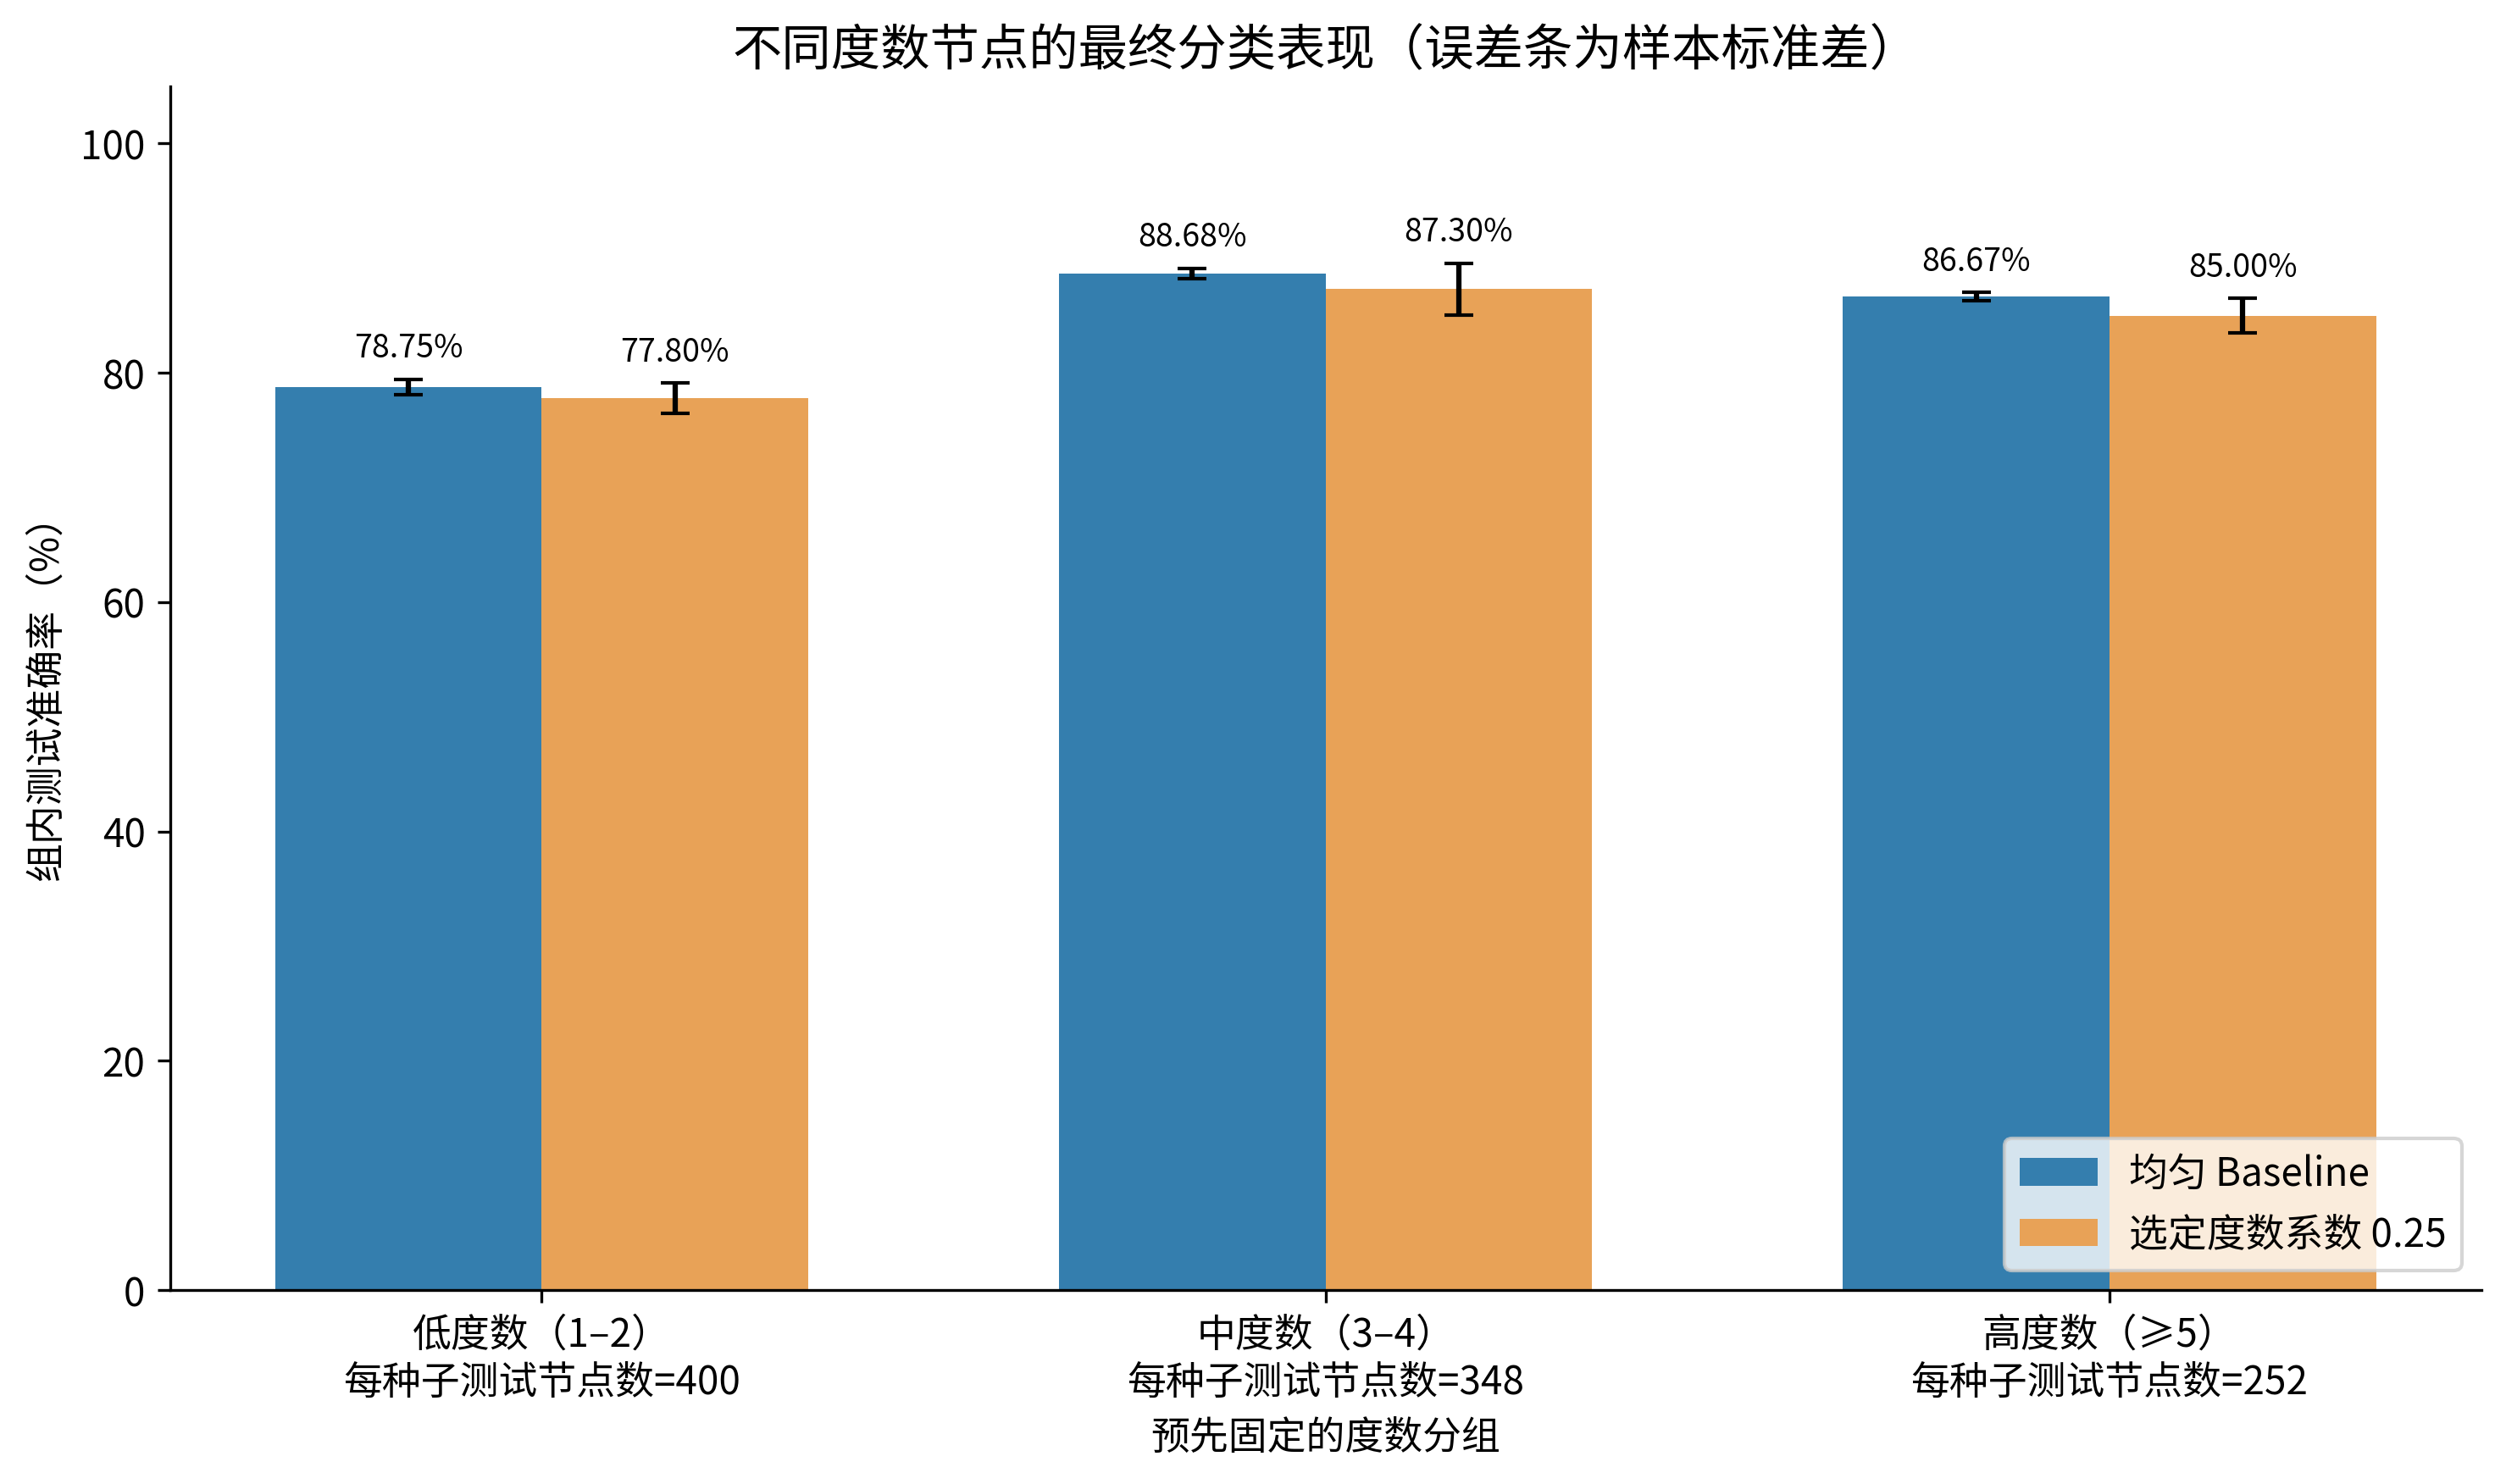
\includegraphics[width=0.90\linewidth]{../figures/M2/degree_classification.png}
\caption{控制组与0.25的度数组测试准确率。柱为五种子均值，误差条为样本SD；每seed固定使用400、348、252个测试节点。分组边界未使用测试标签。}\label{fig:m2-groups}
\end{figure}

五个种子共用同一public split，因此例如低度数组的2000次评价仍来自固定400个节点，不构成2000个独立测试样本。各组规模不均，组内差异仅用于描述哪些节点集合可能受影响，不足以证明单一作用机制。

\subsection{Loss与训练开销}
图\ref{fig:m2-loss}及表\ref{tab:m2-cost}显示，控制组最后100轮的平均SCE为0.402125，0.25方案为0.414893；0.5和1.0分别为0.425383和0.442083。本次没有“降低重建Loss但分类退化”的现象，重建数值也未改善。由于采样使参与损失的节点分布改变，不同方案的SCE并非同一组等难度目标上的泛化误差，不能用其绝对大小代替分类评价。
\begin{figure}[tbp]
\centering
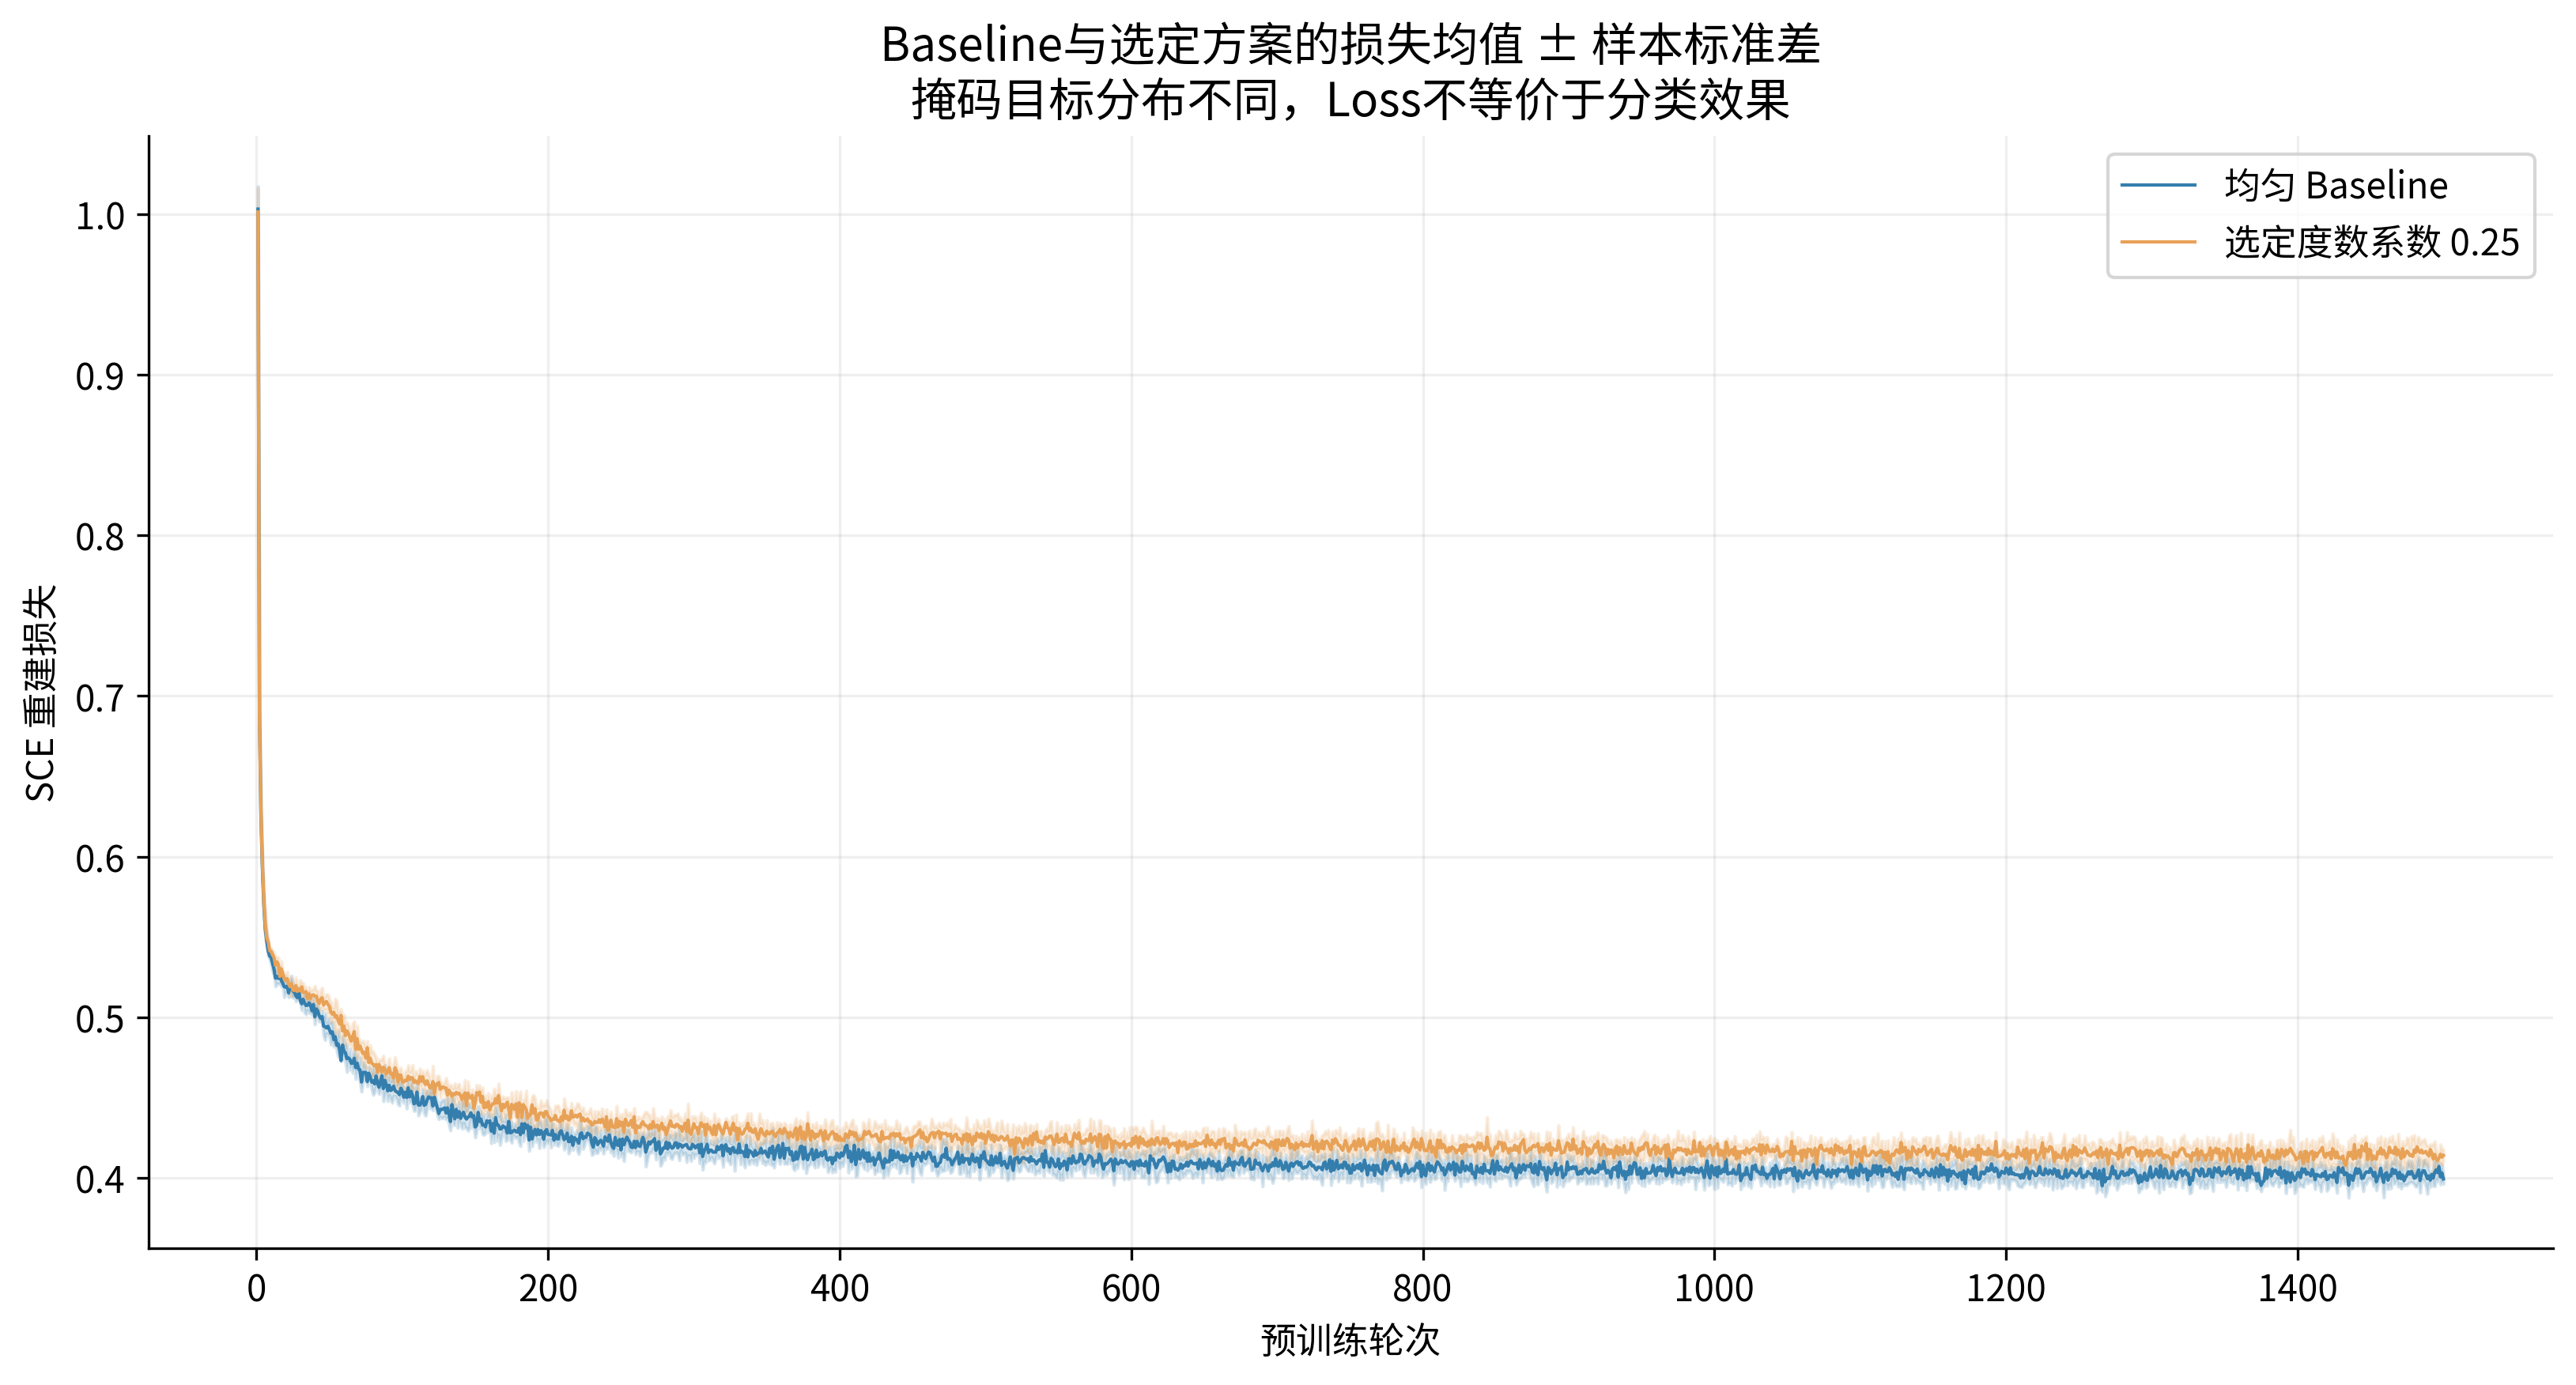
\includegraphics[width=0.90\linewidth]{../figures/M2/loss_curves.png}
\caption{M2控制组与0.25的预训练SCE。曲线为逐轮五种子均值，阴影为样本SD，两者使用不同掩码目标分布。}\label{fig:m2-loss}
\end{figure}
\begin{table}[tbp]
\centering\small
\caption{M2训练过程统计。末100轮Loss先对各seed取均值再跨seed平均；时间为worker均值，峰值为PyTorch allocated张量显存的跨seed平均。}\label{tab:m2-cost}
\begin{tabular}{rrrr}\toprule
$\alpha_d$ & 末100轮SCE & 时间/s & 峰值显存/MiB\\\midrule
0 & 0.402125 & 26.993 & 472.73\\
0.25 & 0.414893 & 28.219 & 472.73\\
0.5 & 0.425383 & 27.538 & 472.69\\
1.0 & 0.442083 & 29.380 & 472.73\\\bottomrule
\end{tabular}
\end{table}

M2时间包含数据、初始化、预训练、全部Probe和保存，不包含模块导入、启动前GPU资源检查与后续最终测试。0.25比控制组均值增加约1.23秒，但服务器负载、CPU采样和日志校验均会影响计时，且并非专门的性能基准，不能据此精确归因采样开销。峰值张量显存约473MiB，未包含所有CUDA上下文或其他用户进程。M1计时包含导入，与M2边界不同，不作跨批次加速比较。

\section{讨论与局限性}\label{sec:limitations}
\subsection{可能的机制解释}
度数加权的直觉是高度数节点拥有更多重建上下文，但它同时改变谁提供可见特征、谁承担重建目标。高度数节点更频繁地被遮蔽，可能使较多邻居失去有用的输入信号；低度数节点则因固定总预算而更少成为重建目标，可能削弱对这些节点的直接监督。均匀掩码的潜在优势是对每个节点提供近似相同的重建机会，不主动以度数重加权训练目标。

此外，SCE要求恢复原始特征方向，下游线性分类要求表示中类别信息可被简单分离，二者并非同一目标。某类节点可被邻域较容易地重建，不意味着提高其重建频率就会增强分类相关信息。重掩码、邻域相关性和标签同质性也可能共同影响结果。上述均是可能原因，本实验没有对可见邻居比例、分组重建误差或各机制分别进行消融，不能将平均下降归因于其中某一条。当前证据支持的是“掩码分布改变且分类均值下降”，而非对退化原因的因果证明。

\subsection{实验范围与协议限制}
实验仅包含Cora、五个种子及三个预设正向系数，没有跨数据集、负系数或其他权重函数的证据。以同一验证划分上的五种子均值选参仍属于有限的开发集探索，虽然测试没有反馈调参，也不提供跨数据集泛化保证。度数组的样本量和人数不均、相同测试节点在不同seed中重复使用，限制了对局部差异的统计解释。

M1与M2使用相同网络、数据和训练预算，但M2为控制策略分支的随机消耗而采用独立CPU选点。M2均匀组84.20\%与M1的83.98\%之间存在随机协议及GPU差异，不能将0.22个百分点解释为度数算法或工程适配提升。有效算法比较来自M2内部重新训练的配对控制组。

M2全部训练和前九次最终测试在L40上进行。最后一个0.25/seed4模型启动测试前，L40剩余显存不足8GiB，资源检查拒绝启动；之后补测入口的一次源码搜索路径错误也发生在任何测试前向之前。修正后在显存充足的共享A40上完成该模型唯一一次最终推断，保留失败日志和设备记录，没有重训、重选系数或重复其他九次测试。该模型的82.8\%包含不同推断设备的潜在浮点影响，应披露为限制；为避免额外测试，本文没有再次推断来估计其大小。

随机种子、cuDNN标志及RNG轨迹的一致性只能控制部分随机因素，不能保证PyG scatter等GPU归约位级确定。原论文20次初始化与本文五次、DGL与PyG历史实现、软件和硬件环境也不同。本文不强行进行显著性检验，不将一次小幅正差或平均负差解释为充分统计证据。该负结果说明预设度数策略在本次条件下没有达到改善目标，不证明所有度数策略或应用场景均无效。

\section{总结}\label{sec:conclusion}
本文围绕GraphMAE的节点特征掩码、GAT编码、重掩码解码与SCE目标，完成了Cora上的课程级部分复现。官方PyG固定版本在五种子下得到83.98\%的测试均值和1.056882个百分点的样本标准差，与原论文84.2\%的报告均值接近，但初始化次数与环境差异使其不能视为完全相同协议的复现。

在自主实验中，本文只改变掩码节点采样，设计并实现固定预算的度数加权无放回策略。二十次训练完成后，验证集在三个正向系数中选择0.25；最终其测试均值82.92\%低于同协议均匀控制组84.20\%，平均配对变化为$-1.28$个百分点。实际掩码统计证明高度数节点被更频繁选中，但三类度数组的平均分类准确率均下降，末100轮SCE也更高。

这些结果表明，增加某类节点的重建机会不必然改善下游表示。本文的贡献在于对一个明确、可实现的采样假设进行受控检验并保留负结果，而非提出已证实有效的新算法。结论受单数据集、少量种子、有限参数候选及数值非确定性限制，相关机制解释仍需独立证据支持。

\bibliographystyle{unsrtnat}
\bibliography{references}
\ifincludeFullAppendix
\clearpage
\appendix
\begingroup
\setstretch{1.0}
\fontsize{9}{11}\selectfont
% Generated by scripts/generate_appendices.py. Whole files only.
\section{完整自编代码及配置}
以下按文件完整导入；论文正文、方法图和参考文献源文件在附录D列出并随电子附件提供。
\subsection*{\texttt{\detokenize{reports/check_sources.py}}}
\appendixfile{../reports/check_sources.py}
\subsection*{\texttt{\detokenize{scripts/analyze_m1.py}}}
\appendixfile{../scripts/analyze_m1.py}
\subsection*{\texttt{\detokenize{scripts/analyze_m2.py}}}
\appendixfile{../scripts/analyze_m2.py}
\subsection*{\texttt{\detokenize{scripts/bootstrap_m0.py}}}
\appendixfile{../scripts/bootstrap_m0.py}
\subsection*{\texttt{\detokenize{scripts/build_report.py}}}
\appendixfile{../scripts/build_report.py}
\subsection*{\texttt{\detokenize{scripts/check_m1_protocol.py}}}
\appendixfile{../scripts/check_m1_protocol.py}
\subsection*{\texttt{\detokenize{scripts/check_m2.py}}}
\appendixfile{../scripts/check_m2.py}
\subsection*{\texttt{\detokenize{scripts/export_agent_logs.py}}}
\appendixfile{../scripts/export_agent_logs.py}
\subsection*{\texttt{\detokenize{scripts/final_check.py}}}
\appendixfile{../scripts/final_check.py}
\subsection*{\texttt{\detokenize{scripts/generate_appendices.py}}}
\appendixfile{../scripts/generate_appendices.py}
\subsection*{\texttt{\detokenize{scripts/m2_masking.py}}}
\appendixfile{../scripts/m2_masking.py}
\subsection*{\texttt{\detokenize{scripts/package_delivery.py}}}
\appendixfile{../scripts/package_delivery.py}
\subsection*{\texttt{\detokenize{scripts/plot_m1.py}}}
\appendixfile{../scripts/plot_m1.py}
\subsection*{\texttt{\detokenize{scripts/plot_m2.py}}}
\appendixfile{../scripts/plot_m2.py}
\subsection*{\texttt{\detokenize{scripts/preflight_m1.py}}}
\appendixfile{../scripts/preflight_m1.py}
\subsection*{\texttt{\detokenize{scripts/resume_m2_test.py}}}
\appendixfile{../scripts/resume_m2_test.py}
\subsection*{\texttt{\detokenize{scripts/run_m1.py}}}
\appendixfile{../scripts/run_m1.py}
\subsection*{\texttt{\detokenize{scripts/run_m2.py}}}
\appendixfile{../scripts/run_m2.py}
\subsection*{\texttt{\detokenize{scripts/setup_env.py}}}
\appendixfile{../scripts/setup_env.py}
\subsection*{\texttt{\detokenize{scripts/smoke_test.py}}}
\appendixfile{../scripts/smoke_test.py}
\subsection*{\texttt{\detokenize{scripts/validate_m0.py}}}
\appendixfile{../scripts/validate_m0.py}
\subsection*{\texttt{\detokenize{scripts/verify_m1.py}}}
\appendixfile{../scripts/verify_m1.py}
\subsection*{\texttt{\detokenize{scripts/verify_m2.py}}}
\appendixfile{../scripts/verify_m2.py}
\subsection*{\texttt{\detokenize{configs/requirements.in}}}
\appendixfile{../configs/requirements.in}
\subsection*{\texttt{\detokenize{configs/requirements.lock.txt}}}
\appendixfile{../configs/requirements.lock.txt}
\subsection*{\texttt{\detokenize{configs/smoke.json}}}
\appendixfile{../configs/smoke.json}
\section{主要Codex任务与最终回答}
\subsection*{M0}
\paragraph*{Prompt}
\appendixtext{../agent_logs/M0/prompt.md}
\paragraph*{Response}
\appendixtext{../agent_logs/M0/response.md}
\subsection*{M1}
\paragraph*{Prompt}
\appendixtext{../agent_logs/M1/prompt.md}
\paragraph*{Response}
\appendixtext{../agent_logs/M1/response.md}
\subsection*{M2}
\paragraph*{Prompt}
\appendixtext{../agent_logs/M2/prompt.md}
\paragraph*{Response}
\appendixtext{../agent_logs/M2/response.md}
\subsection*{M3.1}
\paragraph*{Prompt}
\appendixtext{../agent_logs/M3_1/prompt.md}
\paragraph*{Response}
\appendixtext{../agent_logs/M3_1/response.md}
\subsection*{M3.2}
\paragraph*{Prompt}
\appendixtext{../agent_logs/M3_2/prompt.md}
\paragraph*{Response}
\appendixtext{../agent_logs/M3_2/response.md}
\section{项目Skill与Agent工作流}
\subsection*{\texttt{\detokenize{SKILL.md}}}
\appendixtext{../SKILL.md}
\subsection*{\texttt{\detokenize{AGENT_WORKFLOW.md}}}
\appendixtext{../AGENT_WORKFLOW.md}
\section{第三方源码、数据与电子材料索引}
官方仓库为\url{https://github.com/THUDM/GraphMAE}，保留MIT许可证。
正式PyG版本Commit：\par\noindent\texttt{9127f25e01aa5ba1cca68b746284aeb7ab2b4850}。
DGL审计版本Commit：\par\noindent\texttt{b14f080c919257b495e3cb6474286d5252d6a635}。
两个完整源码目录和Git bundle电子提供，不重复打印原作者源码。
\begin{itemize}
\item 数据：\texttt{data/cora/}，8个raw与3个processed文件，预处理见实验环境章节。
\item 实验：\texttt{results/raw/M0/}、\texttt{M1/}、\texttt{M2/}及\texttt{results/processed/}，含真实日志、配置、预测、必要权重与汇总。
\item 图片：\texttt{figures/M1/}、\texttt{figures/M2/}和\texttt{reports/figures/}，字体二进制不打包；已渲染图片可直接编译。
\item 第三方逐文件清单：\texttt{results/raw/M0/pyg\_tree.txt}与\texttt{main\_tree.txt}。
\item 依赖：\texttt{configs/requirements.lock.txt}；项目历史管理文档电子保留。
\item 全包校验：ZIP内\texttt{FILE\_MANIFEST.json}与\texttt{SHA256SUMS.txt}；根目录\texttt{BUILD\_ON\_WINDOWS.md}说明本地编译。
\end{itemize}
以下论文及方法图源码电子完整提供，避免重复打印已呈现的正文：
\begin{itemize}
\item \texttt{\detokenize{reports/figures/degree_masking_scheme.tex}}
\item \texttt{\detokenize{reports/main.tex}}
\item \texttt{\detokenize{reports/references.bib}}
\item \texttt{\detokenize{reports/sections/01_introduction.tex}}
\item \texttt{\detokenize{reports/sections/02_related.tex}}
\item \texttt{\detokenize{reports/sections/03_method.tex}}
\item \texttt{\detokenize{reports/sections/04_protocol.tex}}
\item \texttt{\detokenize{reports/sections/05_reproduction.tex}}
\item \texttt{\detokenize{reports/sections/06_degree_masking.tex}}
\item \texttt{\detokenize{reports/sections/07_results.tex}}
\item \texttt{\detokenize{reports/sections/08_discussion.tex}}
\item \texttt{\detokenize{reports/sections/09_conclusion.tex}}
\end{itemize}

\endgroup
\fi
\end{document}
